\documentclass{article}

% Recommended, but optional, packages for figures and better typesetting:
\usepackage{microtype}
\usepackage{graphicx}
\usepackage{subcaption}
\usepackage{booktabs}
\usepackage{svg}
% hyperref makes hyperlinks in the resulting PDF.
\usepackage{hyperref}

% Attempt to make hyperref and algorithmic work together better:
\newcommand{\theHalgorithm}{\arabic{algorithm}}

% Use the following line for the initial blind version submitted for review:
\usepackage{icml2026}

% For preprint, use
% \usepackage[preprint]{icml2026}

% If accepted, instead use the following line for the camera-ready submission:
% \usepackage[accepted]{icml2026}

\usepackage{amsmath}
\usepackage{amssymb}
\usepackage{amsfonts}
\usepackage{mathtools}
\usepackage{amsthm}
\usepackage{bm}
\usepackage{bbm}
\usepackage{enumitem}
\usepackage{float}
\usepackage{placeins}
\usepackage{mdframed}
\usepackage[nameinlink]{cleveref}
\usepackage{tikz}
\usepackage{pgfplots}
\usepackage[acronym]{glossaries}

\pgfplotsset{compat=1.18}

% macros.tex
% Package imports live in main.tex to respect the ICML 2026 template order.
\usetikzlibrary{arrows.meta,positioning,calc,fit,decorations.pathreplacing}

\DeclareMathOperator*{\argmin}{argmin}
\DeclareMathOperator*{\argmax}{argmax}
\numberwithin{equation}{section}

% General macros
\newcommand{\nodes}{\mathcal{V}}
\newcommand{\edges}{\mathcal{E}}
\newcommand{\sites}{\mathcal{U}}
\newcommand{\dom}{\mathcal{X}}
\newcommand{\Conf}{\Omega}
\newcommand{\Neighbourhood}{\mathcal{N}}
\newcommand{\Unif}{\mathcal{U}}
\newcommand{\1}{\mathbbm{1}}
\newcommand{\embed}{\bm{\varphi}}
\newcommand{\energy}{E} 

\DeclareMathOperator{\Categorical}{Categorical}

% acronyms
\glsdisablehyper
\newacronym{fm}{FM}{flow matching}
\newacronym{dm}{DM}{diffusion model}
\newacronym{gem}{GEM}{graph energy matching}
\newacronym{gw}{GW}{Gromov–Wasserstein}
\newacronym{gwot}{GWOT}{Gromov–Wasserstein optimal transport}
\newacronym{mh}{MH}{Metropolis–Hastings}
\newacronym{ebm}{EBM}{energy-based model}
\newacronym{ot}{OT}{optimal transport}
\newacronym{mcmc}{MCMC}{Markov chain Monte Carlo}
\newacronym{jko}{JKO}{Jordan–Kinderlehrer–Otto}


% The \icmltitle you define below is probably too long as a header.
% Therefore, a short form for the running title is supplied here:
\icmltitlerunning{Graph Energy Matching}

\begin{document}

\twocolumn[
\icmltitle{Graph Energy Matching:\\
Transport-Aligned Energy-Based Modeling for Controllable Graph Generation}
%Controllable(?) Graph Generation with Transport‑Aligned Discrete Proposals}
  \vskip 0.05in
  {\small\textcolor{red}{\textbullet\ Page limit is 8; we currently exceed it and will move material to the appendix.\\
  \textbullet\ ICML abstract 23rd of January, paper 28th of January}}
  \begin{icmlauthorlist}
    \icmlauthor{Anonymous}{anon}
  \end{icmlauthorlist}

\icmlaffiliation{anon}{Anonymous Institution}
\icmlcorrespondingauthor{Anonymous Author}{anon.email@domain.com}

  \icmlkeywords{Energy-based models, graph generation, optimal transport}

  \vskip 0.3in
]

\printAffiliationsAndNotice{}  % no special notice (required even if empty)

\begin{abstract}

Energy-based models (EBMs) provide a natural mechanism for controllable generation in discrete domains by composing objectives and constraints into an energy function. However, such methods tend to struggle with poorly constrained energies that lie outside the support of the data  distribution, with a wide fidelity gap between them and the diffusion-based generative models. We introduce Graph Energy Matching (GEM), a controllable generative framework for graphs that makes EBMs competitive for generative modeling in discrete spaces. Specifically, GEM learns a single, permutation-invariant potential for (i) transport-aligned guidance from a simple source distribution to the data distribution, (ii) likelihood refinement in the data manifold. GEM is motivated by a discrete Jordan–Kinderlehrer–Otto perspective and uses permutation-invariant minibatch couplings. Further, GEM employs a two-regime discrete MCMC procedure for sampling. (i) A transport phase that applies gradient-informed multi-site edits to reach high-probability regions rapidly (ii) followed by a Metropolis–Hastings mixing phase with geometry-aware proposals. We show that not only does GEM achieve strong unconditional generation quality on molecular graph benchmarks, but it also enables controlled generation at inference time by augmenting the learned energy with additional constraints.
\end{abstract}






%MAIN TEXT
\section{Introduction}
\label{sec:introduction}

Generative modeling of discrete structured objects, such as graphs, is a central challenge across many scientific and industrial applications, including drug discovery and materials design.

The key difficulty arises from the combinatorial complexity of the underlying data distribution, where domain-specific constraints and patterns significantly shape high-probability regions.
%
Current state-of-the-art models for unconditional graph generation predominantly rely on discrete diffusion~\citep{vignac2022digress} or continuous-time Markov chains~\citep{campbell2024generative,qinmadeira2024defog}, translating samples from simple reference distributions into complex graph structures. Although effective in generating realistic unconditional samples, these methods struggle when enforcing user-specified properties or constraints, as the guidance typically occurs off-manifold—where property regressors and conditioning functions are inherently less reliable.
%\end{mdframed}

Energy-based models (EBMs) offer a complementary perspective that naturally addresses these limitations~\citep{hinton2002training}. EBMs represent the data distribution implicitly through a single scalar energy function, enabling the direct incorporation of constraints, priors, or property-based objectives at inference time without retraining~\citep{du2019implicit, du2025learning}. Particularly for graph generation, EBMs have the advantage that permutation invariance and graph-structured constraints can be explicitly and elegantly integrated into the energy. Yet, historically, EBMs have struggled with sample quality, primarily due to poor sampling efficiency in discrete, combinatorial domains, as exemplified by existing methods like GraphEBM~\citep{liu2021graphebm}. Consequently, discrete EBMs have predominantly served as scoring models for out-of-distribution detection rather than as competitive generative samplers~\citep{wu2023energy,fuchsgruber2024energy}.


Energy Matching~\citep{balcerak2025energy} bridges these perspectives in continuous spaces by learning a time-independent potential that simultaneously (i) guides samples from a reference distribution toward data, and (ii) defines a Boltzmann-like density near data via contrastive refinement. This regularizes energies off-support while retaining the compositional advantages of energy-based models (EBMs). However, the continuous formulation still relies on explicit, time-indexed sampling schedules (via ordinary or stochastic differential equations; ODEs/SDEs) to trigger exploration and mixing. Extending Energy Matching to discrete graph spaces, we remove this explicit time dependence entirely, instead using local edits within a Markov Chain Monte Carlo (MCMC) sampler. Here, an energy-dependent criterion implicitly switches between exploration (transport) and refinement regimes, naturally matching the combinatorial structure of graphs. Effective graph-based generation thus requires symmetry-aware transport supervision and efficient discrete sampling strategies.

\Gls{jko} provides a variational framework for optimization in spaces of probability measures, where each
step balances an energy against a distance (or discrepancy) rooted in \gls{ot}, such as the Wasserstein
metric~\citep{lanzetti2025firstorder,lanzetti2024variational,terpin2024learning}. This perspective motivates OT-inspired transport supervision under a given geometry.
For graphs, \gls{gw}-type costs offer permutation-respecting
comparisons~\citep{krzakala2024any2graph}. At the same time, computing exact Wasserstein geodesics is
typically impractical at scale. Importantly, stochastic interpolants~\citep{albergoBuildingNormalizingFlows2023} with data-dependent couplings~\citep{albergo2024stochastic} provide a principled way to work with tractable, possibly suboptimal couplings; i.e., minibatch coupling induces practically useful paths that guide sampling toward data-supported regions without requiring exact solutions to optimal transport. This motivates using efficient approximate graph couplings to supervise global guidance toward high-probability regions, combined with local refinement steps to ensure effective exploration and validity.
\begin{figure*}[t]
\centering

% Okabe–Ito palette
\definecolor{otColor}{RGB}{230,159,0}   % orange: OT
\definecolor{mhColor}{RGB}{0,114,178}   % blue:   MH
\tikzset{state/.style={circle,draw,minimum size=11mm,inner sep=0pt}}

\begin{tikzpicture}[>=Stealth, every node/.style={font=\small}, node distance=1.7cm]

% Transport phase nodes (orange shade)
\node[state,fill=orange!20]                    (pi0b) {$\pi_{0}$};
\node[state,fill=orange!20,right=of pi0b]      (pi1b) {$\pi_{1}$};
\node[right=of pi1b]                           (dots1b) {$\dots$};
\node[state,fill=orange!20,right=of dots1b]    (pikb) {$\pi_{k}$};

% Phase-transition divider
\draw[densely dashed,line width=1.2pt] ($(pikb.east)+(0.10,0.95)$) -- ($(pikb.east)+(0.10,-0.95)$);

% Mixing phase nodes (blue shade)
\node[right=1.2cm of pikb]                       (dots2b) {$\dots$};
\node[state,fill=blue!15,right=1.0cm of dots2b]  (pidatab) {$\pi_{\text{data}}$};
\node[right=2mm of pidatab]                      (eqb) {$=$};
\node[state,fill=blue!15,right=2mm of eqb]       (pistb) {$\pi_{\theta}$};

% Transport arrows
\draw[->,very thick,draw=otColor,shorten <=7pt,shorten >=7pt] (pi0b) -- (pi1b);
\draw[->,very thick,draw=otColor,shorten <=7pt,shorten >=7pt] (pi1b) -- (dots1b);
\draw[->,very thick,draw=otColor,shorten <=7pt,shorten >=7pt] (dots1b) -- (pikb);

% MH arrows
\draw[->,very thick,draw=mhColor,shorten <=7pt,shorten >=7pt] (pikb) -- (dots2b);
\draw[->,very thick,draw=mhColor,shorten <=7pt,shorten >=7pt] (dots2b) -- (pidatab);

% Annotation for gradient-informed transport
\node[below=10pt of dots1b,align=center,font=\scriptsize]
      {greedy discrete proposals on samples\\(direction $-\nabla_x V_{\theta}(x)$ $\leftrightarrow$ transport map direction)};


% Annotation for discrete proposals + MH
\node[below=10pt of dots2b,align=center,font=\scriptsize,xshift=36pt]
      {local, geometry-aware, $\nabla_x V_\theta(x)$-informed jumps\\+ MH acceptance};

% Phase annotations
\node[align=center,above=1mm of pi1b]
      {\textbf{Transport Phase}\\[-1pt]\scriptsize samples far from data manifold: $V_{\theta}(x) \gg V_{\text{data}}^{\text{mean}}$};

\node[align=center,above=1mm of pidatab]
      {\textbf{Mixing Phase}\\[-1pt]\scriptsize samples near data manifold: $V_{\theta}(x) \sim V_{\text{data}}^{\text{mean}}$};

% Self-loop at stationary state
\draw[->,thick,draw=mhColor]
  ($(pistb.east)+(2pt,3pt)$) arc[start angle=160,end angle=-160,radius=8pt];

\end{tikzpicture}

\caption{Illustration of GEM sampling, a two-phase MCMC method. Sampling alternates between a transport phase, where gradient-informed, greedy proposals rapidly move samples toward regions of high probability, and a mixing phase employing MH acceptance to ensure correct stationary distribution and efficient mixing between modes. \textbf{Color key:} transport (\textcolor{otColor}{orange}), MH (\textcolor{mhColor}{blue}).}

\label{fig:sampling-regimes}
\end{figure*}


\begin{mdframed}[hidealllines=true,backgroundcolor=blue!5]
\paragraph{Contributions.}
We propose \acrlong{gem}\footnote{Code will be released upon acceptance.}, a state-of-the-art discrete energy-based model for graphs, achieving unconditional generation quality competitive with leading discrete diffusion models. GEM combines:
(i) global transport guidance through permutation-invariant graph couplings under a relaxed OT geometry,
(ii) a learned, time-independent potential explicitly defining a Gibbs distribution over graphs, and
(iii) efficient geometry-aware local edit proposals combined with Metropolis–Hastings sampling.

GEM uniquely retains the compositional and controllable properties of energy-based models, enabling inference-time incorporation of constraints or objectives into the energy. Additionally, its explicit energy structure naturally facilitates computing graph geodesics—minimum-energy edit paths aligned with the learned data geometry—and enables state-of-the-art conditional generation. GEM also achieves state-of-the-art generation of novel graphs by editing existing samples.
\end{mdframed}

\section{Preliminaries: Energy Matching and JKO }

Energy matching learns a scalar potential \( V_\theta:\mathcal{X}\to\mathbb{R} \), parameterized by \(\theta\), on a continuous data space \(\mathcal{X}\). It simultaneously serves two complementary roles: (i)~off-manifold guidance, directing samples toward the data manifold via the gradient field \(-\nabla_x V_\theta\), and (ii)~near-equilibrium refinement, characterizing the data distribution on the manifold as an \gls{ebm} with Gibbs density \(\propto \exp(-V_\theta(x))\).

These roles separate model learning into a \emph{global} transport-alignment and a \emph{local} density-refinement term. A simple time-dependent temperature schedule to switch between these regimes, e.g., \(\epsilon(t)=0\) for \(t<1\) (transport) and \(\epsilon(t)=1\) for \(t\ge 1\) (mixing), (i) injects exploration, (ii) mitigates mode collapse, and (iii) stabilizes sampling from the Gibbs distribution \(\propto \exp(-V_\theta(x))\).

Energy Matching can be understood through an optimization-in-probability-spaces perspective, expressed via the \gls{jko}) scheme from density $\rho_t$ to $\rho_{t+\Delta t}$:
\begin{align}
\label{jko_em}
\rho_{t+\Delta t}
&=
\arg\min_{\rho}\;
\frac{1}{2\Delta t}\,\inf_{\gamma\in\Gamma(\rho_t,\rho)}\mathbb{E}_{(x,y)\sim\gamma}[\,c(x,y)\,]\nonumber\\
&\quad+\;\int V_\theta(y)\,\rho(y)\,\mathrm{d}y\nonumber\\
&\quad+\;\epsilon(t)\int \rho(y)\log\rho(y)\,\mathrm{d}y,
\end{align}
where the cost function \( c(x,y) \) measures the amount of displacement when transporting mass from \(x\) to \(y\), and constitutes a design choice---in continuous spaces typically chosen as \( c(x,y)=\|x - y\|^2 \).

The coupling \(\gamma\in\Gamma(\rho,\rho_t)\) is a joint distribution that characterizes a transport plan: it precisely describes how mass from the current configuration \(\rho_t\) is relocated to form the new distribution \(\rho\). Intuitively, \(\gamma(x,y)\) encodes ``how much mass from each location \(x\sim\rho_t\) is transported to each new location \(y\sim\rho\)'', thus determining the optimal reassignment of mass that minimizes the expected transportation cost \(\mathbb{E}_{(x,y)\sim\gamma}[\,c(x,y)\,]\).

\paragraph{Off-manifold transport guidance.}
Based on first-order optimality conditions in Wasserstein space~\citep{lanzetti2024variational,lanzetti2025firstorder} applied to the functional in~\cref{jko_em}, Energy Matching defines two clear learning objectives. Given tractably coupled pairs \((x,y)\sim\gamma\) (e.g., obtained via minibatch matching rather than solving for the globally optimal coupling), we associate \(x_0\) with the noise/source distribution (\(\rho_{0}\)) and \(x_1\) with the data/target distribution (\(\rho_{\mathrm{data}}\)). Intermediate points are sampled as \(x_t=(1-t)x_0+t x_1\) for \(t\sim\Unif([0,1])\). Defining the empirical transport direction \(v=x_1 - x_0\), the \(V_\theta\) is trained via a flow-like objective:
\begin{equation}
\mathcal{L}_{\mathrm{Flow}}
=
\mathbb{E}_{(x,y)\sim\gamma,\,t\sim\Unif([0,1])}\big[\|\nabla_{x_t} V_\theta(x_t) + v\|^2\big].
\end{equation}

\paragraph{Near-equilibrium energy refinement.}
At equilibrium (\(t\to\infty\) in Eq.~\eqref{jko_em} and in the mixing regime \(\epsilon(t)=1\)), the stationary distribution induced by \(V_\theta\) is given by:
\begin{equation}
\rho_{t\to\infty}(x)\propto \exp(-V_\theta(x)).
\end{equation}

Refinement of the equilibrium density is achieved using the contrastive loss (CL) (see Appendix \ref{app:energy-refinement}):
\begin{equation}
\label{eq:cl}
\mathcal{L}_{\mathrm{CL}}
=
\mathbb{E}_{x^{+}\sim \rho_{\mathrm{data}}}[V_\theta(x^{+})]
-
\mathbb{E}_{x^{-}\sim\operatorname{sg}(\rho_{t\to\infty})}[V_\theta(x^{-})],
\end{equation}
where negative samples \(x^{-}\) are generated via Langevin dynamics initialized either from the source or from data, with gradients stopped (\(\operatorname{sg}\)) during sampling. Training begins with an initial warm-up phase using only \(\mathcal{L}_{\mathrm{Flow}}\), followed by joint optimization of:
\begin{equation}
\mathcal{L}(\theta)=\mathcal{L}_{\mathrm{Flow}}(\theta)+\lambda_{\mathrm{CL}}\,\mathcal{L}_{\mathrm{CL}}(\theta).
\end{equation}

\paragraph{Sampling (two regimes).}
Sampling starts from a transport-aligned drift and switches to refinement via an effective temperature
$\epsilon(t)$. In continuous time, this corresponds to the time-inhomogeneous \gls{sde}
\begin{equation}
\label{em_sde}
\mathrm{d}x_t
=
-\nabla_{x_t} V_\theta(x_t)\,\mathrm{d}t
+\sqrt{2\,\epsilon(t)}\,\mathrm{d}W_t,
\end{equation}
which reduces to an \gls{ode} when $\epsilon(t)=0$ and becomes stochastic as $\epsilon(t)\to 1$.
In practice, sampling corresponds to explicitly integrating \cref{em_sde} over a fixed time interval.

\subsection{Regressor-guided Diffusion}
Both DeFoG~\citep{qinmadeira2024defog} and Variational Flow Matching (VFM)~\citep{eijkelboom2024vfm,eijkelboom2025controlledvfm} achieve controllable graph diffusion by conditioning transitions on noise-dependent regressors predicting desired properties. Formally, these regressors approximate conditional distributions of graph properties $y$ given intermediate noisy graph states $x_t$, i.e., $\rho(y\mid x_t,t)$ or $\rho_t(y\mid x_t)$. Further details and empirical analyses illustrating how prediction accuracy behaves at different noise levels are provided in Appendix~\ref{app:regressor-noise}. {\color{red}\textbf{TODO: move to appendix/baselines.}}

\section{Graph Energy Matching}
\label{sec:gem}
We extend continuous Energy Matching methods to discrete graph spaces through a novel transport-aligned discrete proposal tailored specifically for discrete probability distributions. Our formulation employs an energy-based switching mechanism that clearly separates \emph{transport} and \emph{mixing} sampling regimes without requiring explicit indexing of time or noise levels. Sampling is efficiently facilitated through deterministic greedy proposals in the transport regime or stochastic gradient-informed proposals during mixing, alongside an annealing strategy to efficiently generate novel samples from optionally given data samples via incremental edits. The sampler uses a temperature $\epsilon$ to control stochasticity: the transport regime is the deterministic $\epsilon\to 0$ limit, while the mixing regime uses $\epsilon>0$.

\paragraph{Graph representation.} 
We consider a discrete state space $\mathcal{X}:=\big(\mathcal{X}_{\mathrm{node}}\big)^{n}\times\big(\mathcal{X}_{\mathrm{edge}}\big)^{\binom{n}{2}}$ to represent undirected graphs. A graph $x\in \mathcal{X}$ contains a set of $n$ nodes $\mathcal{V}=\{1,\dots,n\}$ and edges $\mathcal{E}$ defining the connectivity between these nodes. Each node $i\in\mathcal{V}$ has a node class $x_i \in \mathcal{X}_{\mathrm{node}}$ (e.g.\ an atom type), and each edge $(i,j)\in\mathcal{E}$ has an edge class $x_{ij}\in\mathcal{X}_{\mathrm{edge}}$ (e.g.\ a bond type). The edge space $\mathcal{X}_{\mathrm{edge}}$ includes an element indicating the absence of an edge.




The graph $x:=\big(x_\mathcal{V},x_\mathcal{E}\big)$ consists of $x_\mathcal{V}$ and $x_\mathcal{E}$ denoting categorical node and edge features, respectively, and are defined as
\begin{equation}
x_\mathcal{V}  :=[x_i]_{i=1}^n\in(\mathcal{X}_{\mathrm{node}})^n;\quad
x_\mathcal{E}  :=[x_{ij}]_{ i<j}\in\big(\mathcal{X}_{\mathrm{edge}}\big)^{\binom{n}{2}}\nonumber
\end{equation}

We embed the node and edge categorical feature vectors $x_\mathcal{V}$ and $x_\mathcal{E}$ using a real-valued one-hot encoding and treat them as continuous features via
\[
\phi_{\mathcal{V}} :\mathcal{X}_{\mathrm{node}}\to\mathbb{R}^{l_{\mathrm{node}}};\quad
\phi_{\mathcal{E}} :\mathcal{X}_{\mathrm{edge}}\to\mathbb{R}^{l_{\mathrm{edge}}}
\]
where $l_{\mathrm{node}}=|\mathcal{X}_{\mathrm{node}}|$ and $l_{\mathrm{edge}}=|\mathcal{X}_{\mathrm{edge}}|$ denote the numbers of node and edge classes, respectively. We denote the real-valued node features $\hat{x}_{\mathcal{V}}\in\mathbb{R}^{n l_{\mathrm{node}}}$ and edge features $\hat{x}_{\mathcal{E}}\in\mathbb{R}^{\binom{n}{2}l_{\mathrm{edge}}}$, and the corresponding graph representation 
$\hat{x}\in\mathbb{R}^d$, where $d=n l_{\mathrm{node}}+\binom{n}{2}l_{\mathrm{edge}}$, as:
\begin{equation}
\hat{x}_\mathcal{V}:=\oplus_{i=1}^n \phi_\mathcal{V}(x_i);\quad
\hat{x}_\mathcal{E}:=\oplus_{i<j}\phi_\mathcal{E}(x_{ij});\quad
\hat{x}:=\hat{x}_\mathcal{V}\oplus \hat{x}_\mathcal{E}. \nonumber
\end{equation}
where $\oplus$ denotes the element-wise concatenation operation.
We parameterize the energy as $V_\theta(x):=\tilde V_\theta(\hat{x})$, differentiable with respect to
the continuous embedding $\hat{x}$.

\paragraph{Local and Permutation-Invariant Geometries.} The potential $V_\theta$ is permutation-invariant by construction (Appendix~\ref{app:perm-invariance}), so the geometry used for pairing should also respect node relabelings. Here, $\sigma\in S_n$ acts on node indices and induces a relabeling of the graph: $(\sigma\cdot x)_i=x_{\sigma(i)}$ and $(\sigma\cdot x)_{ij}=x_{\sigma(i)\sigma(j)}$. We measure local discrepancies in the embedding by
\begin{equation}\label{eq:loc-cost}
c_{\mathrm{loc}}(x,y)
\;\coloneqq\;
\lambda_\mathcal{V}\|\hat{x}_{\mathcal{V}}-\hat{y}_{\mathcal{V}}\|^2_2
+
\lambda_\mathcal{E}\|\hat{x}_{\mathcal{E}}-\hat{y}_{\mathcal{E}}\|^2_2,
\end{equation}
with $\lambda_\mathcal{V},\lambda_\mathcal{E}>0$ scaling node and edge contributions. This is the
embedding-space cost $c(x,y):=\tilde c(\hat{x},\hat{y})$, and it is differentiable in both
arguments. To compare graphs in a permutation-invariant way, we lift the local cost by optimizing
over node relabelings to obtain the \gls{fgw} cost \citep{vayer2019optimal}:
\begin{equation}\label{eq:fgw-cost}
c_{\mathrm{FGW}}(x,y)
=
\min_{\sigma\in S_n}
\left\{
c_{\mathrm{loc}}(x,\sigma\cdot y)
\right\}.
\end{equation}
This quantity is used for minibatch pairings and transport supervision. Exact evaluation is
intractable, so we use fast approximations: histogram matching for noisy--clean pairing and
node-matching for molecule--molecule pairing (Appendix~\ref{app:matching}). These pairings map each
source/noise graph $x^0$ to a data graph $x^\mathrm{data}=T(x^0)$ and define displacements
$v=\hat{x}^\mathrm{data}-\hat{x}^0$ that supervise the transport-aligned drift used to train
$-\nabla_{\hat{x}}V_\theta$ (Section~\ref{sec:training}).



\begin{figure}[h]
\centering
\resizebox{0.95\columnwidth}{!}{%
\begin{tikzpicture}[>=Latex, font=\small]

% ---------------- Panel box ----------------
\def\W{11.2}
\def\H{4.9}
\node[font=\small\bfseries] at (\W/2-0.7,\H+0.45)
{Discrete, geometry-aware energy-based proposal (local edits)};

% ---------------- Center + shells ----------------
\coordinate (xhat) at (3.8,1.55);

\pgfmathsetmacro{\rOne}{0.85}
\pgfmathsetmacro{\rTwo}{1.35}
\pgfmathsetmacro{\rThr}{1.85}

\draw[cb_lightgray, dashed, line width=0.7pt] (xhat) circle[radius=\rOne];
\draw[cb_lightgray, dashed, line width=0.7pt] (xhat) circle[radius=\rTwo];
\draw[cb_lightgray, dashed, line width=0.7pt] (xhat) circle[radius=\rThr];

\node[cb_lightgray, font=\scriptsize, align=center] at ($(xhat)+(-2.3,1.2)$)
{distance penalty\\isolines};

\node[cb_lightgray, font=\scriptsize\bfseries] at ($(xhat)+(115:\rOne)+(0.06,-0.24)$) {1 edit};
\node[cb_lightgray, font=\scriptsize\bfseries] at ($(xhat)+(115:\rTwo)+(0.06,-0.26)$) {2 edits};
\node[cb_lightgray, font=\scriptsize\bfseries] at ($(xhat)+(115:\rThr)+(0.06,-0.28)$) {3 edits};

\filldraw[black, fill=cb_red] (xhat) circle (2.2pt);
\node[font=\scriptsize, anchor=north east] at ($(xhat)+(-0.06,-0.12)$) {$\hat{x}$};
\node[cb_lightgray, font=\scriptsize\bfseries, anchor=west] at ($(xhat)+(0.12,-0.02)$) {stay};

% ---------------- Gradient direction ----------------
\pgfmathsetmacro{\gdeg}{30} % degrees
\coordinate (gend) at ($(xhat)+(\gdeg:3.05)$);
\draw[->, ultra thick, cb_green] (xhat) -- (gend);
\node[font=\small\bfseries, anchor=west, cb_green]
  at ($(xhat)+(1.8,1.0)$)
  {$-\nabla_{\hat{x}} V_\theta(\hat{x})$};

% ---------------- Dot area encodes probability ----------------
\pgfmathsetmacro{\A}{2.0}
\pgfmathsetmacro{\B}{1.0}

\pgfmathsetmacro{\sOne}{exp(\A*\rOne - \B*\rOne*\rOne)}
\pgfmathsetmacro{\sTwo}{exp(\A*\rTwo - \B*\rTwo*\rTwo)}
\pgfmathsetmacro{\sThr}{exp(\A*\rThr - \B*\rThr*\rThr)}
\pgfmathsetmacro{\smax}{max(\sOne,max(\sTwo,\sThr))}

\pgfmathsetmacro{\radMin}{0.35}
\pgfmathsetmacro{\radScale}{2.25}

\newcommand{\DrawRing}[3]{%
  \foreach \ang in {#2} {%
    \pgfmathsetmacro{\score}{exp(\A*#1*cos(\ang-\gdeg) - \B*#1*#1)}%
    \pgfmathsetmacro{\p}{\score/\smax}%
    \pgfmathsetmacro{\rad}{\radMin + \radScale*sqrt(\p)}%
    \filldraw[black, fill=#3] ($(xhat)+(\ang:#1)$) circle[radius=\rad pt];
  }%
}

\DrawRing{\rOne}{0,30,60,90,120,150,180,210,240,270,300,330}{cb_blue}
\DrawRing{\rTwo}{15,45,75,105,135,165,195,225,255,285,315,345}{cb_blue}
\DrawRing{\rThr}{0,45,90,135,180,225,270,315}{cb_blue}

% ---------------- Legend + equation (spaced higher) ----------------
\node[draw, rounded corners, fill=white, inner sep=6pt,
      font=\small, anchor=north, align=left]
  at (\W/2 -0.7,\H+0.10)
{$q_\mathrm{mixing}(x\to y)\propto \exp\bigl(
- \lambda^L_{\mathcal{V}}\|\hat{y}_{\mathcal{V}}-\hat{x}_{\mathcal{V}}\|_2^2
- \lambda^L_{\mathcal{E}}\|\hat{y}_{\mathcal{E}}-\hat{x}_{\mathcal{E}}\|_2^2$\\[4pt]
$\quad\quad\quad\quad\quad\quad - \beta^L\,\nabla V_\theta(\hat{x})^\top(\hat{y}-\hat{x})\bigr)$};

% ---------------- Dot area explanation repositioned ----------------
\node[font=\small, anchor=west] at (5.6,1.9)
{dot area $\propto\, q_\mathrm{mixing}(x\to y)$};

\end{tikzpicture}%
}
\caption{\textbf{Proposal Scoring.} Local graph edit proposals with scoring given by $q_\mathrm{mixing}(x\to y)$. The size of dots encodes proposal probabilities. Alignment with the gradient direction increases the probability, while distance penalties discourage larger edits. If the candidate is the origin (stay), we resample to promote exploration. (with equal node/edge weights $\lambda^L_{\mathcal{V}} = \lambda^L_{\mathcal{E}}$ for illustrative purposes)}
\label{fig:proposal-middle-softmax-alpha-half}
\end{figure}



\subsection{Discrete Transport-Aligned Proposal ($\epsilon\to 0$)}{\color{red} TODO: point to details}

\label{proposals}

Given an optimal coupling $\gamma$ (in practice approximated using tractable methods, e.g.,~\cite{albergo2024stochastic,tong2024improving}) and its induced transport map $T$, we assume $T$ admits a consistent representation of the form $y=T(x) \iff \hat{y}=\tilde{T}(\hat{x})$, with $x$ drawn from the source/noise distribution and $y$ from the data distribution, where $\tilde{T}$ is a continuous map that realizes $T$ under the embedding.  Expressing the JKO variational objective from \Cref{jko_em} as an optimization over transport maps (see \Cref{app:jko}) and substituting the time-step parameter $\Delta t$ with the jump step-size $\eta$ yields:
\begin{equation}
\label{eq:new_T}
    T(x)\in\arg\min_{y\in\mathcal{X}}\left\{\frac{1}{2\eta}c(x,y)+V_\theta(y)\right\},
\end{equation}
where $\pi_{k+1}=T_{\#}\pi_k$ denotes the pushforward of $\pi_k$.



Assuming the minimizer $T(x)$ lies in the interior, the first-order optimality condition becomes
\begin{equation}
0 = \left.\nabla_{\hat{y}}\left[\frac{1}{2\eta}\tilde{c}(\hat{x},\hat{y})+\tilde{V}_\theta(\hat{y})\right]\right|_{\hat{y}=\tilde{T}(\hat{x})},
\end{equation}
which implies
\begin{equation}
\nabla_{\hat{y}}\tilde V_\theta\!\left(\tilde T(\hat{x})\right)
\;=\;
-\frac{1}{2\eta}\,
\nabla_{\hat{y}}\tilde c\!\left(\hat{x},\tilde T(\hat{x})\right).
\end{equation}
This optimality condition fully characterizes the solution and can thus be directly employed as a training objective. We utilize this approach in \Cref{sec:training}, incorporating the global, permutation-invariant cost from \Cref{eq:fgw-cost}.

We are now, at sampling, trying to solve \Cref{eq:new_T} given a trained network on the above objective. We want to make the proposal local as to iterate the descent in the potential in more than one-shot such that we can also do a taylor expension on $V(y)$ around x. Rather than controlling the step-size parameter $\eta$, we simplify the (local) greedy proposal by restricting the kernel to exactly $N$ edits per jump. For this proposal we consider the cost to be $c_{\mathrm{loc}}(x,y)$ with $\lambda_\mathcal{V}=\lambda_\mathcal{E}$ which yields fixed costs for every such candidate - which means the cost is constant and can be neglected within the search. Linearizing $V_\theta(y)\approx V_\theta(x)+\Delta\hat{x}^\top\nabla_{\hat{x}} V_\theta(\hat{x})$ around $\hat{x}$, with $\Delta\hat{x}=\hat{y}-\hat{x}$, we deterministically select the top-$N$ candidate edits ranked by steepest descent. Formally, the candidate set $C_N(x)$ is defined as the set of all edits achievable by exactly $N$ discrete modifications (changing/removing edges or changing nodes) starting from state $x$. The greedy  proposal is thus given by:
\begin{gather}
y^*(x) = x + \arg\min_{\Delta x \in C_N(x)} (\Delta\hat{x})^\top\nabla_{\hat{x}} V_\theta(\hat{x}), \\
q_{\text{greedy}}(x\to y) = \delta_{y^*(x)}(y).
\end{gather}

In the transport regime, we project the proposed moves onto directions with strictly negative gradient, rejecting any edits that do not satisfy this condition. It is deterministic. If no candidate edits yield a negative gradient direction, the greedy sampler becomes trapped, prompting a transition to the Langevin-based proposal $q_\mathrm{mixing}$.

\subsection{Discrete Mixing Proposal ($\epsilon>0$).}
Discretizing the dynamics (\Cref{em_sde}) in the embedding space  with temperature $\epsilon$, step size $\eta$, and graphs $x,y \in \mathcal{X}$ yields:
\begin{equation}
q_{\mathrm{mixing}}(x\to y)
\,\propto\,
\exp\left(
-\frac{1}{4\epsilon\eta}\|\hat{y}-\hat{x}+\eta\nabla V_\theta(\hat{x})\|^2
\right).
\end{equation}

Expanding explicitly and dropping terms independent of $\hat{y}$:
\begin{align}
\log q_\mathrm{mixing}(x\to y)
&=
-\frac{1}{4\epsilon\eta}\|\hat{y}-\hat{x}\|^2
- \frac{1}{2\epsilon}\nabla V_\theta(\hat{x})^\top(\hat{y}-\hat{x})\notag\\
&\quad+\text{const.}
\end{align}
The proposal is effectively local because of the distance penalty, although technically it can still propose an arbitrary number of edits. We define Langevin-specific parameters $(\lambda_{\mathcal{V}}^L, \lambda_{\mathcal{E}}^L, \beta^L)$ absorbing all constants (including $\epsilon$, $\eta$, and numerical factors):
\addtocounter{equation}{1}
\begin{align}
&q_\mathrm{mixing}(x\to y)
\;\propto\tag{\theequation}\\
&\quad\exp\!\bigl(
- \lambda_{\mathcal{V}}^L\|\hat{y}_{\mathcal{V}}-\hat{x}_{\mathcal{V}}\|_2^2
- \lambda_{\mathcal{E}}^L\|\hat{y}_{\mathcal{E}}-\hat{x}_{\mathcal{E}}\|_2^2
- \beta^L\,\nabla V_\theta(\hat{x})^\top(\hat{y}-\hat{x})
\bigr).\notag
\end{align}


The resulting kernel can be viewed as a \emph{linearized locally balanced proposal}; related
discrete-gradient samplers appear in~\citep{zanella2020informed, grathwohl2021oops,zhang2022langevin} for particular costs or candidate sets.
Figure~\ref{fig:proposal-middle-softmax-alpha-half} illustrates the resulting geometry-aware proposal
scoring and how gradient alignment competes with distance penalties.

In practice, this Langevin-based proposal is combined with a Metropolis--Hastings acceptance step, ensuring convergence to the target distribution $\pi_\theta(x)\propto\exp(-\beta_{mh} V_\theta(x))$. 

We calibrate the parameters $\beta_{mh}$, $\beta^{L}$, $\lambda_{\mathcal{V}}^{L}$, and $\lambda_{\mathcal{E}}^{L}$ by maximizing the relative likelihood of generated samples compared to the training dataset samples under the learned energy $V_\theta$, directly after the warmup training phase described in \Cref{sec:training}.



In the mixing regime, we accept the stochastic proposal with \gls{mh} probability:
\begin{equation}\label{eq:mh-accept}
\begin{aligned}
\alpha(x,y)
&=\min\left(1,\frac{\pi_\theta(y)\,q_{\mathrm{mixing}}(y\to x)}{\pi_\theta(x)\,q_{\mathrm{mixing}}(x\to y)}\right).\\
\end{aligned}
\end{equation}
This choice
enforces detailed balance:
\begin{equation}\label{eq:mh-detailed-balance}
\begin{aligned}
\pi_\theta(x)\,q_{\mathrm{mixing}}(x\to y)\,\alpha(x,y)
= \\
\pi_\theta(y)\,q_{\mathrm{mixing}}(y\to x)\,\alpha(y,x)
\end{aligned}
\end{equation}
so $\pi_\theta$ is stationary for the mixing dynamics~\citep{metropolis1953equation,hastings1970monte}.
Implementation details of the proposal kernel (factorized logits, temperature annealing, and do-nothing
resampling) are provided in Appendix~\ref{app:sampling-details}.



\subsection{Initializations and proposal schedules.}

\paragraph{Determining the Regime}
\label{switch}
We control the regime through an energy-based binary indicator $s\in\{0,1\}$: $s=0$ selects transport (deterministic $\epsilon\to 0$ limit), while $s=1$ selects mixing (finite $\epsilon>0$). If initialized at noise, the sampler follows deterministic greedy edits guided strictly by negative gradient directions. Transition from transport to mixing occurs when the Markov chain either reaches the target energy (defined as the mean data energy estimated during training) or becomes trapped in a local minimum—no valid gradient-improving edits exist—for all samples, whichever happens first. Once triggered, the sampler enters the stochastic Langevin-based mixing regime. More about proposal schedules in \Cref{init_prop}.

\paragraph{Init.... TODO}
\label{init_prop}
We use two initialization regimes with aligned proposal schedules:
\begin{itemize}[leftmargin=*]
\item \textbf{Noise initialization:} sample the node count from the empirical histogram, then draw node/edge
types uniformly (uniform noise) or from empirical marginals (marginal noise). These start far from
the data distribution, so we run transport with greedy proposals $q_{\text{greedy}}$ until the energy-based switch (see
\Cref{switch}), then enter mixing with the proposal
$q_{\mathrm{mixing}}$. 
\item \textbf{Data initialization:} draw graphs from the training set. We skip transport and start directly in mixing with $q_{\mathrm{mixing}}$, using a higher initial proposal temperature that is annealed before
fixed-temperature mixing (Appendix~\ref{app:sampling-details}).
\end{itemize}
All initializations start near-zero \gls{vun}. Figure~\ref{fig:moses-energy-and-metrics}
summarizes the resulting energy trajectories under noise vs.\ data initialization and the
corresponding proposal regimes.

\begin{figure}[h]
\centering

\begin{tikzpicture}[scale=1.15]
  \draw[->, thick] (0,-0.36) -- (6.2,-0.36);
  \draw[->, thick] (0,-0.36) -- (0,2.6);
  \node[rotate=90] at (-0.7,1.12) {$V_\theta(x)$};
  \node[font=\small\bfseries] at (3.1,2.9) {Energy Trajectories};

  % Axes ticks
  \foreach \x/\lab in {0/0,1.2/100,2.4/200,3.6/300,4.8/400,6.0/500} {
    \draw (\x,-0.36) -- (\x,-0.42);
    \node[below, font=\scriptsize] at (\x,-0.42) {\lab};
  }
  \foreach \y/\lab in {-0.36/-40,0/0,0.9/100,1.8/200,2.475/275} {
    \draw (0,\y) -- (-0.08,\y);
    \node[left, font=\scriptsize] at (-0.1,\y) {\lab};
  }

  % Annealing window (S) - Using TEAL (was Green)
  \draw[decorate, decoration={brace, amplitude=4pt, mirror}, draw=cb_teal] (0.06,0.2) -- (2.10,0.2);
  \node[font=\scriptsize, text=cb_teal] at (1.36,-0.16) {annealed temperature mixing};
  
  % Fixed-temperature window - Using BLUE (was Blue)
  \draw[decorate, decoration={brace, amplitude=4pt, mirror}, draw=cb_blue] (2.28,0.2) -- (5.94,0.2);
  \node[font=\scriptsize, text=cb_blue] at (4.20,-0.16) {fixed-temperature mixing};

  % Bands (range)
    % Noise band (Orange)
    \fill[cb_orange!20] (0,1.78) rectangle (6.0,2.28);
    \draw[cb_orange, line width=0.6pt] (0,2.03) -- (6.0,2.03);
    
    % Data band (Blue)
    \fill[cb_blue!20, opacity=0.5] (0,0.18) rectangle (6.0,0.68);
    \draw[cb_blue, line width=0.6pt] (0,0.43) -- (6.0,0.43);


  % Greedy proposal window - Using RED (was Red)
  \draw[decorate, decoration={brace, amplitude=4pt}, draw=cb_red] (0.06,2.34) -- (2.22,2.34);
  \node[font=\scriptsize, text=cb_red] at (1.14,2.65) {greedy proposals};

  % Trajectories (means + std)
  
  % Noise Initialized (RED)
  \fill[cb_red!20, opacity=0.6] plot[smooth] coordinates {
    (0.0,2.392) (0.7,1.992) (1.3,1.492) (2.1,0.742)
    (2.7,0.732) (3.3,0.732) (4.2,0.732) (5.1,0.732) (6.0,0.732)
  } -- plot[smooth] coordinates {
    (6.0,0.172) (5.1,0.172) (4.2,0.172) (3.3,0.172)
    (2.7,0.172) (2.1,0.182) (1.3,0.932) (0.7,1.432) (0.0,1.832)
  } -- cycle;
  \draw[cb_red, densely dotted, line width=1.1pt] plot[smooth] coordinates {
    (0.0,2.112) (0.7,1.712) (1.3,1.212) (2.1,0.462)
    (2.7,0.452) (3.3,0.452) (4.2,0.452) (5.1,0.452) (6.0,0.452)
  };

  % Data Initialized (TEAL - was Green)
  \fill[cb_teal!30, opacity=0.5] plot[smooth] coordinates {
    (0.0,0.74) (0.4,0.91) (0.9,0.82) (1.4,0.74)
    (2.2,0.72) (3.1,0.71) (4.2,0.71) (5.1,0.71) (6.0,0.71)
  } -- plot[smooth] coordinates {
    (6.0,0.18) (5.1,0.18) (4.2,0.18) (3.1,0.18)
    (2.2,0.18) (1.4,0.18) (0.9,0.26) (0.4,0.35) (0.0,0.18)
  } -- cycle;
  \draw[cb_teal, densely dotted, line width=1.1pt] plot[smooth] coordinates {
    (0.0,0.46) (0.4,0.63) (0.9,0.54) (1.4,0.46)
    (2.2,0.44) (3.1,0.43) (4.2,0.43) (5.1,0.43) (6.0,0.43)
  };

  % Legend
\begin{scope}[shift={(3.3,1.7)}]
  % Noise band (orange): band + constant (solid) reference line
  \draw[fill=cb_orange!20, draw=cb_orange] (0,0) rectangle (0.35,0.18);
  \draw[cb_orange, line width=0.6pt] (0.04,0.09) -- (0.31,0.09);
  \node[anchor=west, font=\scriptsize] at (0.45,0.09) {noise band};

  % Data band (blue): band + constant (solid) reference line
  \draw[fill=cb_blue!20, draw=cb_blue, fill opacity=0.5] (0,-0.28) rectangle (0.35,-0.10);
  \draw[cb_blue, line width=0.6pt] (0.04,-0.19) -- (0.31,-0.19);
  \node[anchor=west, font=\scriptsize] at (0.45,-0.19) {data band};

  % Noise initialized samples (red): band + dotted mean line
  \draw[fill=cb_red!20, draw=cb_red] (0,-0.56) rectangle (0.35,-0.38);
  \draw[cb_red, densely dotted, line width=1.1pt] (0.04,-0.47) -- (0.31,-0.47);
  \node[anchor=west, font=\scriptsize] at (0.45,-0.47) {samples: noise initialized};

  % Data initialized samples (teal): band + dotted mean line
  \draw[fill=cb_teal!30, draw=cb_teal] (0,-0.84) rectangle (0.35,-0.66);
  \draw[cb_teal, densely dotted, line width=1.1pt] (0.04,-0.75) -- (0.31,-0.75);
  \node[anchor=west, font=\scriptsize] at (0.45,-0.75) {samples: data initialized};
\end{scope}

\end{tikzpicture}

\vspace{0.25cm}

\begin{tikzpicture}[xscale=0.99, yscale=1.06]
  \draw[->, thick] (0,0) -- (7.2,0) node[midway, below=14pt] {Inference \glsentryshort{mcmc} steps};
  \draw[->, thick] (0,0) -- (0,3.35);
  \node[rotate=90] at (-0.9,1.6) {Fraction$\uparrow$};

  % Title
  \node[font=\small\bfseries] at (3.5,3.55) {Validity \& Novelty Trajectories};

  % Axes ticks
  \foreach \x/\lab in {0/0,1.4/100,2.8/200,4.2/300,5.6/400,7.0/500} {
    \draw (\x,0) -- (\x,-0.06);
    \node[below, font=\scriptsize] at (\x,-0.06) {\lab};
  }
  \foreach \y/\lab in {0/0.00,0.8/0.25,1.6/0.50,2.4/0.75,2.88/0.90,3.2/1.00} {
    \draw (0,\y) -- (-0.08,\y);
    \node[left, font=\scriptsize] at (-0.1,\y) {\lab};
  }

  % Validity (Data Init) - Using TEAL
  \draw[cb_teal, thick] plot[smooth] coordinates {
    (0.0,3.20) (0.1,1.40) (0.2,0.55) (0.3,0.26) (0.6,0.22)
    (1.0,0.30) (1.4,0.42) (1.8,0.70) (2.2,1.05) (2.6,1.40)
    (3.0,1.70) (3.4,2.00) (3.8,2.25) (4.2,2.45) (4.6,2.60)
    (5.0,2.72) (5.6,2.86) (6.2,3.06) (6.8,3.075) (7.0,3.088)
  };

  % Novelty (Data Init) - Using TEAL (Dashed)
  \draw[cb_teal, thick, dashed] plot[smooth] coordinates {
    (0.0,0.00) (0.1,0.05) (0.2,0.25) (0.3,0.80) (0.4,1.60)
    (0.5,2.72) (1.0,2.45) (1.5,1.70) (2.0,2.05) (2.5,2.30)
    (3.0,2.45) (3.5,2.60) (4.0,2.70) (4.5,2.78) (5.0,2.85)
    (5.5,2.90) (6.0,2.95) (6.5,2.98) (7.0,3.00)
  };

  % Validity (Noise Init) - Using RED
  \draw[cb_red, thick] plot[smooth] coordinates {
    (0.0,0.00) (0.6,0.08) (1.0,0.32) (1.4,1.12) (1.8,2.24)
    (2.2,2.60) (2.6,2.72) (3.0,2.80) (4.2,2.88) (5.6,2.92) (7.0,2.944)
  };
  % Novelty (Noise Init) - Using RED (Dashed)
  \draw[cb_red, thick, dashed] plot[smooth] coordinates {
    (0.0,3.20) (1.4,3.187) (2.8,3.174) (4.2,3.162) (5.6,3.149) (7.0,3.136)
  };

  % Legend
  \begin{scope}[shift={(3.3,0.15)}]
    \draw[fill=white, draw=cb_gray] (0,0) rectangle (3.6,1.4);
    
    % Noise Init (Red)
    \draw[cb_red, thick] (0.15,1.15) -- (0.6,1.15);
    \node[anchor=west, font=\scriptsize] at (0.7,1.15) {Validity (noise initialized)};
    \draw[cb_red, thick, dashed] (0.15,0.85) -- (0.6,0.85);
    \node[anchor=west, font=\scriptsize] at (0.7,0.85) {Novelty (noise initialized)};
    
    % Data Init (Teal)
    \draw[cb_teal, thick] (0.15,0.45) -- (0.6,0.45);
    \node[anchor=west, font=\scriptsize] at (0.7,0.45) {Validity (data initialized)};
    \draw[cb_teal, thick, dashed] (0.15,0.15) -- (0.6,0.15);
    \node[anchor=west, font=\scriptsize] at (0.7,0.15) {Novelty (data initialized)};
  \end{scope}
\end{tikzpicture}
\caption{\footnotesize \textbf{Energy and Sampling Trajectories.} Top: energy evolution for noise- vs.\ data-initialized chains, with mean $\pm$ 1 std bands and reference levels at $\mathbb{E}_{x\sim \pi_\mathrm{data}}[V_\theta(x)]$ and $\mathbb{E}_{x\sim \pi_0}[V_\theta(x)]$. Noise-initialized chains use greedy proposals to reach the data distribution; data-initialized chains use temperature annealing (low initial $\beta_{\mathrm{mh}}$, gradually increasing) to recover novelty.
 Bottom: validity and novelty trajectories for data-initialized (teal) and noise-initialized (red) chains over inference steps. Uniqueness $\approx$100\%.}
\label{fig:moses-energy-and-metrics}
\vspace{-5pt}
\end{figure}

\subsection{Training objectives}
\label{sec:training}

\paragraph{Noise and Data Interpolation via Minibatch coupling.}
Given minibatches \( x^0 \sim \pi_0 \) and \( x^\mathrm{data} \sim \pi_\mathrm{data} \) where $\pi_0$ is the uniform noise and $\pi_{data}$ is the data distribution respectively. We pair samples using a permutation-invariant approximation of \( c_{\mathrm{FGW}}(x^0,x^\mathrm{data}) \) described in \Cref{sec:gem}, via histogram matching (\Cref{app:matching}), and solving for a transport map \( T \) induced by the minibatch coupling, using the \texttt{POT} solver \citep{Flamary2021}.
 Each source graph $x^0$ is paired with a data graph $x^\mathrm{data}=T(x^0)$.
% In all experiments involving our method, we initialize from a uniform noise distribution $\pi_0$.

Crucially, we utilize $c_{\mathrm{FGW}}$ solely to select optimal pairs based on global structural similarity (e.g., node and edge counts). %Once paired, we rely on the isotropy of the uniform source: since the noise graph lacks intrinsic node ordering, any node permutation is statistically equivalent. We therefore treat the sampled node ordering of $x^0$ as implicitly aligned with the paired $x^{\mathrm{data}}$ via the identity permutation. 
% This approach is compatible with our architecture because $V_\theta$ is permutation-invariant by construction (\Cref{app:perm-invariance}), ensuring the learned energy landscape is independent of the specific stochastic node labeling.
Denote their embeddings by $\hat{x}^0$ and $\hat{x}^\mathrm{data}$. Define the
displacement in the embedding space as $v=\hat{x}^\mathrm{data}-\hat{x}^0$.
We sample a \emph{discrete} interpolant $x^t:=(x^t_\mathcal{V},x^t_\mathcal{E})$, where $x_\mathcal{V}^t:= [x_i^t]_{i=1}^n$ and $x_\mathcal{E}^t := [x_{ij}^t]_{i<j}$ by independently sampling each node and edge from the endpoint graphs.
\begin{eqnarray}
x_i^t \sim \operatorname{Cat}\Big((1-t)\,\phi_\mathcal{V}\big(x_i^0\big) + t\,\phi_\mathcal{V}\big(x_i^{\mathrm{data}}\big)\Big)\\
x_{ij}^t \sim \operatorname{Cat}\Big((1-t)\,\phi_\mathcal{E}\big(x_{ij}^0\big) + t\,\phi_\mathcal{E}\big(x_{ij}^{\mathrm{data}}\big)\Big)
\end{eqnarray}
% \end{equation}
where $\operatorname{Cat}$ denotes categorical sampling. Let $\hat{x}^t$ be the continuous embedding of the discrete graph $x^t$ via $\phi_\mathcal{V},\phi_\mathcal{E}$ (\Cref{sec:gem}). While this embedding resides in a continuous ambient space, training is conducted solely on discrete graphs $x \in \mathcal{X}$, as sampling proposals are concerning discrete jumps. The continuous embedding thus mainly facilitates gradient computation of $\nabla_{\hat{x}_t} V_\theta(\hat{x}^t)$ to guide these discrete transitions.



\paragraph{Objectives.}
We use the optimality condition derived in \Cref{proposals} to construct a flow-like loss ($\mathcal{L}_{\text{Flow}}$). We set the JKO step-size parameter $\eta=1$. Consequently, the optimality condition $\nabla_{\hat{x}} \tilde{V_\theta}(\hat{x}) = - \frac{1}{2 \eta}\nabla_{\hat{x}} \tilde{c}(\hat{x},\hat{y})$ from \eqref{eq:optimality} implies that the negative energy gradient should match the displacement vector $v$ pointing towards the data. %While the pairing is determined by global signatures,
The training objective minimizes the cost ($c_{\text{loc}}$) along the interpolation path:
\begin{align}
\mathcal{L}_{\text{Flow}}(\theta)
&=
\mathbb{E}_{(x^0,x^\mathrm{data})\sim\tilde{\gamma},\,t\sim\Unif([0,1])}\left[
\|\nabla_{\hat{x}_t} \tilde{V}_\theta(\hat{x}^t)+v\|_2^2
\right],\\
\mathcal{L}_{\text{CL}}(\theta)
&=
\mathbb{E}_{x^{+}\sim \pi_\mathrm{data}}[\tilde{V}_\theta(\hat{x}^{+})]
-\mathbb{E}_{x^{-}\sim \text{sg}\,(\pi_\theta)}[\tilde{V}_\theta(\hat{x}^{-})].
\label{eq:cl}
\end{align} 
The contrastive loss $\mathcal{L}_{\text{CL}}$~\cite{hinton2002training} (see \Cref{app:energy-refinement} for the derivation) leverages the discrete proposals introduced in \Cref{proposals} and \Cref{proposals_lang} to efficiently sample from the model distribution.
 We minimize:
\begin{equation}
\min_\theta\;
\mathcal{L}_{\text{Flow}}(\theta)
+\lambda_{\text{CL}}\,
\mathcal{L}_{\text{CL}}(\theta).
\end{equation}


We perform a warm-up phase of $N_{\mathrm{warmup}}$ training iterations using only $\mathcal{L}_{\text{Flow}}$ before introducing $\mathcal{L}_{\text{CL}}$. This serves two purposes: first, consistent with the intuition from the continuous formulation~\citep{balcerak2025energy}, it yields higher-quality negatives for contrastive learning; second, it allows us to \emph{temporarily} freeze the network after warm-up, solely to calibrate the mixing-phase sampler hyperparameters $(\beta_{\mathrm{mh}}, \beta^L, \lambda_{\mathcal V}^L, \lambda_{\mathcal E}^L)$ required by $\mathcal{L}_{\text{CL}}$. Specifically, we tune these hyperparameters to minimize the energy of samples generated by the fixed $V_\theta$, which is equivalent to maximizing their relative likelihood.

To approximate samples from \( \pi_\theta \) required by \(\mathcal{L}_{\text{CL}}\), we run Markov chains initialized in equal proportions from uniform noise and data samples.
(See \Cref{app:exp-setup} for detailed hyperparameters.) We outline high-level algorithms:
\begin{algorithm}[H]
\caption{GEM Training}
\small
\begin{algorithmic}[1]
\STATE {\bfseries Input:} $N_{\text{CL}}, N_{\text{warmup}}, \lambda_{\text{CL}}$, step $i=0$
\WHILE{$V_\theta$ not converged}
    \STATE Sample $(\xzero,\xdata)\sim\pizero\times\pidata$ (via SOLVER), $t\sim\mathcal{U}(0,1)$
    \STATE $x^t\sim \operatorname{Cat}\big((1 - t)\hat{x}^0 + t\hat{x}^{\text{data}}\big)$
    \STATE $\mathcal{L}_{\text{Flow}}=\|\nabla\tilde{V}_\theta(\hat{x}^t)+(\hat{x}^{\text{data}}-\hat{x}^0)\|^2$
    \IF{ $i>N_{\text{warmup}}$}
        \STATE $x \sim \text{GEM Sampling}(V_\theta) \hfill \leftarrow\ \text{Algorithm~2}$
        \STATE $\mathcal{L}_{\text{CL}}=\mathbb{E}[\tilde{V_\theta}(\hat{x}^{\text{data}})]-\mathbb{E}[\tilde{V_\theta}(\hat{x})]$
    \ELSE
        \STATE $\mathcal{L}_{\text{CL}}=0$
    \ENDIF
    \STATE \textbf{optimizer\_step}($\mathcal{L}_{\text{Flow}}+\lambda_{\text{CL}}\mathcal{L}_{\text{CL}}$) 
    \STATE $i=i+1$
\ENDWHILE
\end{algorithmic}
\end{algorithm}

\begin{algorithm}[H]
\caption{GEM Sampling}
\small
\begin{algorithmic}[1]
\STATE {\bfseries Input:} $V_\theta$, $N_{\text{CL}}$, $V_\text{th}=\mathbb{E}_{\pidata}[\Vtheta]$
\STATE Init. $x\sim\pizero$ (or $\pidata$)
\WHILE{$\Vtheta(x)>V_\text{th}$ {\bfseries and} $x$ not stuck}
    \STATE $x\sim \qgreedy(x\to y)$
\ENDWHILE
\FOR{$k=1$ {\bfseries to} $N_{\text{CL}}$}
    \STATE $x\sim \text{MH-step}(\qmixing(x\to y))$
\ENDFOR
\STATE {\bfseries Return} $x$
\end{algorithmic}
\end{algorithm}
\vspace{-1em}
\section{Experiments}
\label{sec:experiments}

We report unconditional generation on MOSES in the main text and on QM9 in
Appendix~\ref{app:qm9-uncond}, conditional generation under property targets (logP, logS, QED, TPSA), and
geodesic comparisons in the learned space. By convention, on QM9 we report novelty separately from
$V.U.$: the dataset is small and novelty is often far from 1.0, so we include a dedicated novelty
column to show it is comparable and to avoid biasing \gls*{fcd} there.
We report validity (RDKit-sanitized non-empty SMILES), uniqueness (distinct SMILES among valid),
novelty (unique valid molecules not in the training split), and $V.U.N.$ for the fraction satisfying
all three. We also report \gls*{fcd}, a ChemNet feature-space distance between generated and MOSES
molecules (lower is better). We consider two initialization regimes. \textbf{Noise Initialization}
(standard for diffusion models) starts from easy-to-sample noise; the main challenge is to reach
chemically valid molecules, while novelty is often already high. \textbf{Data Initialization}
(available to energy-based models) starts from molecules drawn from the training dataset; the main
challenge is to make non-trivial edits that increase novelty while preserving chemical validity.
In practice, Noise Initialization uses \textbf{uniform noise} (node count from the empirical
histogram, node/edge types uniform) or \textbf{marginal noise} (node count from the empirical
histogram, node/edge types from empirical marginals), while Data Initialization uses \textbf{training
data} samples; sampling can be run with diffusion/CTMC dynamics or MCMC.
MOSES is a large-scale molecular dataset (about 1.5M molecules), while QM9 is a smaller benchmark
focused on low-mass molecules. We use MOSES to stress-test sample quality at scale and QM9 as a
compact setting for comparison.
%
A concise conceptual summary of the baselines used in our experiments is provided in
Appendix~\ref{app:baselines}, and the experimental setup is detailed in Appendix~\ref{app:exp-setup}.

\subsection*{Unconditional generation}
\paragraph{MOSES: Baselines vs.\ GEM.}
Table~\ref{tab:uncond-moses} reports unconditional metrics on MOSES; QM9 results are in
Appendix~\ref{app:qm9-uncond} (Table~\ref{tab:uncond-qm9}).
Figure~\ref{fig:moses-energy-and-metrics} reports annealed-proposal metrics on MOSES. Across both
Noise Initialization and Data Initialization, GEM improves V.U.N.\ and \gls*{fcd}.
Validity, novelty, and uniqueness can be
improved post-hoc via rejection sampling, so diffusion baselines already reach strong V.U.N., but
\gls*{fcd} is less amenable to such correction; we see a clear gap on MOSES. The step curves in
Figure~\ref{fig:moses-vun-steps} show rapid early gains with diminishing returns as steps increase,
and Figure~\ref{fig:moses-energy-and-metrics} highlights the distinct trajectories under Noise vs.\
Data Initialization.
\begin{table}[h]
\centering
\small
\textbf{MOSES} ($\sim$1.5M molecules)\\[2pt]
\begin{tabular}{lcc}
\toprule
Method & V.U.N. $\uparrow$ & \gls*{fcd} $\downarrow$ \\
\midrule
Training samples (MOSES) & 0.0 & 0.09 \\
\midrule
\multicolumn{3}{l}{\textit{Noise Initialization}} \\
\midrule
GraphEBM$^*$~\citep{liu2021graphebm} & 8.12 & 9.83 \\
VFM$^*$~\citep{eijkelboom2024vfm} & 81.39 & 2.71 \\
DeFoG$^*$~\citep{qinmadeira2024defog} & 82.21 & 1.95 \\
\textbf{GEM (Ours)} & \textbf{85.61} & \textbf{1.50} \\
\midrule
\multicolumn{3}{l}{\textit{Data Initialization}} \\
\midrule
GraphEBM$^*$~\citep{liu2021graphebm} & 32.16 & 7.31 \\
\textbf{GEM (Ours)} & \textbf{89.81} & \textbf{0.76} \\
\bottomrule
\end{tabular}
\caption{\footnotesize \textbf{Unconditional Generation.} MOSES results grouped by initialization.
$V.U.N.$ is the valid-unique-novel fraction (higher is better); \gls*{fcd} measures the distance
between generated and MOSES molecules in ChemNet feature space (lower is better). $^*$ reproduced
with the same backbone as DeFoG~\citep{qinmadeira2024defog}; EBMs use a small energy head. Architecture
details are in Appendix~\ref{app:perm-invariance}. 25k generations. Budget of 1000 inference steps.}
\label{tab:uncond-moses}
\end{table}

A schematic of MCMC evolution for GEM on QM9 and MOSES is shown in Appendix~\ref{app:sampling}
(Figure~\ref{fig:appendix-mcmc-traj}).

\begin{figure}[h]
\centering
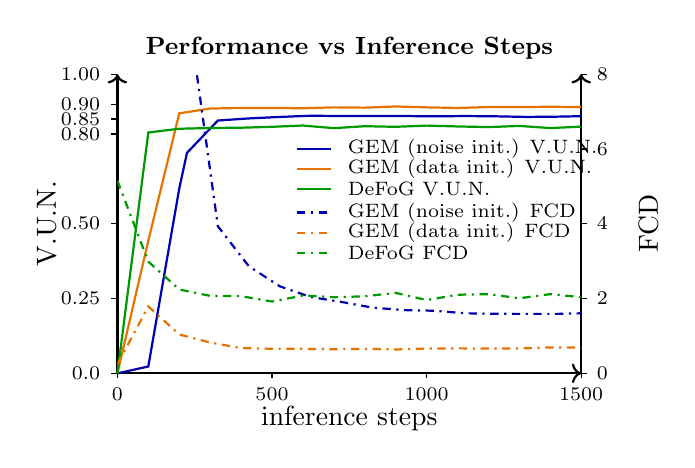
\begin{tikzpicture}[scale=0.95]
  \draw[->, thick] (0,0) -- (6.2,0) node[midway, below=8pt] {inference steps};
  \draw[->, thick] (0,0) -- (0,4.0);
  \node[rotate=90] at (-0.95,2.0) {V.U.N.};
  \draw[->, thick] (6.2,0) -- (6.2,4.0);
  \node[rotate=90] at (7.1,2.0) {FCD};

  % Title
  \node[font=\small\bfseries] at (3.1,4.35) {Performance vs Inference Steps};

  % Axes ticks
  \foreach \x/\lab in {0/0,2.067/500,4.133/1000,6.200/1500} {
    \draw (\x,0) -- (\x,-0.06);
    \node[below, font=\scriptsize] at (\x,-0.06) {\lab};
  }
  \foreach \y/\lab in {0/0.0,1.0/0.25,2.0/0.50,3.2/0.80,3.4/0.85,3.6/0.90,4.0/1.00} {
    \draw (0,\y) -- (-0.08,\y);
    \node[left, font=\scriptsize] at (-0.1,\y) {\lab};
  }
  \foreach \y/\lab in {0/0,1.0/2,2.0/4,3.0/6,4.0/8} {
    \draw (6.2,\y) -- (6.28,\y);
    \node[right, font=\scriptsize] at (6.28,\y) {\lab};
  }
  % Noise initialization (warmup + DLangevin)
  \draw[blue!70!black, thick] plot coordinates {
    (0.000,0.000) (0.413,0.092) (0.827,2.472) (0.930,2.948) (1.343,3.380)
    (1.757,3.408) (2.170,3.428) (2.583,3.444) (2.997,3.440) (3.410,3.440)
    (3.823,3.440) (4.237,3.436) (4.650,3.440) (5.063,3.436) (5.477,3.428)
    (5.890,3.432) (6.200,3.438)
  };

  % Data initialization (annealed)
  \draw[orange!90!black, thick] plot coordinates {
    (0.000,0.000) (0.413,1.772) (0.827,3.476) (1.240,3.540) (1.653,3.548)
    (2.067,3.548) (2.480,3.544) (2.893,3.556) (3.307,3.552) (3.720,3.568)
    (4.133,3.556) (4.547,3.548) (4.960,3.560) (5.373,3.560) (5.787,3.564)
    (6.200,3.560)
  };

  % DeFoG
  \draw[green!60!black, thick] plot coordinates {
    (0.000,0.000) (0.413,3.220) (0.827,3.270) (1.240,3.280) (1.653,3.284)
    (2.067,3.296) (2.480,3.313) (2.893,3.278) (3.307,3.304) (3.720,3.296)
    (4.133,3.312) (4.547,3.301) (4.960,3.292) (5.373,3.308) (5.787,3.279)
    (6.200,3.298)
  };

  % FCD (right axis)
  \begin{scope}
    \clip (0,0) rectangle (6.2,4.0);
    \draw[blue!70!black, thick, dash dot] plot coordinates {
      (0.413,8.184) (0.827,4.961) (0.930,4.952) (1.343,1.966) (1.757,1.432)
      (2.170,1.164) (2.583,1.021) (2.997,0.954) (3.410,0.879) (3.823,0.846)
      (4.237,0.837) (4.650,0.803) (5.063,0.796) (5.477,0.795) (5.890,0.795)
      (6.200,0.803)
    };
    \draw[orange!90!black, thick, dash dot] plot coordinates {
      (0.000,0.122) (0.413,0.895) (0.827,0.520) (1.240,0.412) (1.653,0.338)
      (2.067,0.329) (2.480,0.328) (2.893,0.323) (3.307,0.328) (3.720,0.319)
      (4.133,0.332) (4.547,0.334) (4.960,0.333) (5.373,0.332) (5.787,0.347)
      (6.200,0.344)
    };
    \draw[green!60!black, thick, dash dot] plot coordinates {
      (0.000,2.575) (0.413,1.494) (0.827,1.121) (1.240,1.036) (1.653,1.032)
      (2.067,0.960) (2.480,1.041) (2.893,1.018) (3.307,1.030) (3.720,1.076)
      (4.133,0.980) (4.547,1.051) (4.960,1.059) (5.373,1.004) (5.787,1.059)
      (6.200,1.018)
    };
  \end{scope}

  % Legend
  \begin{scope}[shift={(2.25,1.35)}]
    \draw[blue!70!black, thick] (0.15,1.65) -- (0.6,1.65);
    \node[anchor=west, font=\scriptsize] at (0.7,1.65) {GEM (noise init.) V.U.N.};
    \draw[orange!90!black, thick] (0.15,1.38) -- (0.6,1.38);
    \node[anchor=west, font=\scriptsize] at (0.7,1.38) {GEM (data init.) V.U.N.};
    \draw[green!60!black, thick] (0.15,1.11) -- (0.6,1.11);
    \node[anchor=west, font=\scriptsize] at (0.7,1.11) {DeFoG V.U.N.};
    \draw[blue!70!black, thick, dash dot] (0.15,0.80) -- (0.6,0.80);
    \node[anchor=west, font=\scriptsize] at (0.7,0.80) {GEM (noise init.) FCD};
    \draw[orange!90!black, thick, dash dot] (0.15,0.53) -- (0.6,0.53);
    \node[anchor=west, font=\scriptsize] at (0.7,0.53) {GEM (data init.) FCD};
    \draw[green!60!black, thick, dash dot] (0.15,0.26) -- (0.6,0.26);
    \node[anchor=west, font=\scriptsize] at (0.7,0.26) {DeFoG FCD};
  \end{scope}
\end{tikzpicture}
\caption{\footnotesize \textbf{V.U.N. and FCD vs Steps.} V.U.N. (higher is better) and FCD (lower is better) versus inference steps on MOSES for GEM noise initialization (uniform) with greedy warmup proposal, GEM data initialization with annealed proposal, and DeFoG (marginal noise).}
\label{fig:moses-vun-steps}
\end{figure}











\paragraph{QM9.}
QM9 unconditional metrics are reported in Appendix~\ref{app:qm9-uncond}
(Table~\ref{tab:uncond-qm9}).

\subsection*{Conditional generation}
We evaluate conditional generation under molecular property constraints (e.g., logP, QED).
We train a property regressor \(f_\phi\) (GraphTransformer) for differentiable guidance and define a
conditioned energy \(V_\theta^{\mathrm{cond}}(x)=V_\theta(x)+\lambda_{\mathrm{prop}}\|f_\phi(x)-y^\star\|^2\),
then run the same proposal kernel $q_\theta(x\!\to\!y)$ using \(-\nabla_x V_\theta^{\mathrm{cond}}(x)\),
with the Metropolis--Hastings acceptance ratio modified accordingly. For fairness, all methods use
noise-conditioned regressors; GEM also admits clean regressors, so we report a clean-regressor
ablation in Appendix~\ref{app:regressor-noise} (Figure~\ref{fig:regressor-noise},
Table~\ref{tab:regressor-ablations}). Noise-conditioned regressors are more reliable on noisy or
invalid graphs (and we often must traverse such regions to move between modes), so they provide more
stable guidance. Baselines follow their standard marginal-noise regressors, while GEM uses
uniform-noise conditioning (our training noise), with all other settings matched. We choose targets
(e.g., logS $\ge$ -2.25, logP $\le$ 1.5, QED $\ge$ 0.9, TPSA $\le$ 50) so that unconditional MOSES
samples satisfy the constraint at roughly a 20\% rate, yielding comparable difficulty across
properties.
Table~\ref{tab:moses-conditional} reports single-property conditioning results, and
Appendix~\ref{app:baselines} summarizes joint constraints (Table~\ref{tab:moses-conditional-joint}).
GEM maintains strong validity, uniqueness, and novelty while improving constraint satisfaction
relative to baselines.
GEM draws a candidate pool of size $N_{\mathrm{select}}$ from the training set, ranks by the
precomputed property values, and initializes the $B$ inference chains with the top-$B$ molecules
that satisfy the condition; this takes virtually no time because the training-set properties are
cached.

\begin{table*}[t]
\centering
\small
\textbf{MOSES} ($\sim$1.5M molecules)\\[2pt]
\begingroup
\setlength{\tabcolsep}{3pt}
\begin{tabular}{lcc cc cc cc}
\toprule
Method
& \multicolumn{2}{c}{Condition: logS $\ge$ -2.25}
& \multicolumn{2}{c}{Condition: \acrshort{qed} $\ge$ 0.9}
& \multicolumn{2}{c}{Condition: \acrshort{tpsa} $\le$ 50}
& \multicolumn{2}{c}{Condition: logP $\le$ 1.5} \\
\cmidrule(lr){2-3} \cmidrule(lr){4-5} \cmidrule(lr){6-7} \cmidrule(lr){8-9}
& \glsentryshort{cvun} $\uparrow$ & \glsentryshort{cvu} $\uparrow$
& \glsentryshort{cvun} $\uparrow$ & \glsentryshort{cvu} $\uparrow$
& \glsentryshort{cvun} $\uparrow$ & \glsentryshort{cvu} $\uparrow$
& \glsentryshort{cvun} $\uparrow$ & \glsentryshort{cvu} $\uparrow$ \\
\midrule
Training samples (MOSES) & 0 & 0.24 & 0 & 0.16 & 0 & 0.21 & 0 & 0.15 \\
\midrule
\multicolumn{9}{l}{\textit{Noise Initialization}} \\
\midrule
G-\gls{vfm}$^*$~\citep{eijkelboom2025controlledvfm} & 0.72 & 0.75 & 0.26 & 0.28 & 0.72 & 0.80 & 0.70 & 0.74 \\
DeFoG$^*$~\citep{qinmadeira2024defog} & 0.74 & 0.79 & 0.26 & 0.31 & 0.77 & \textbf{0.82} & 0.78 & 0.82 \\
\textbf{\gls{gem} (Ours)} & \textbf{0.80} & \textbf{0.81} & \textbf{0.40} & \textbf{0.40} & \textbf{0.80} & 0.81 & \textbf{0.85} & \textbf{0.85} \\
\bottomrule
\end{tabular}
\endgroup
\vspace{0.15cm}
\caption{\footnotesize \textbf{Property Conditioning.} MOSES conditional generation under property constraints. \gls{cvun} is the fraction meeting the condition and valid, unique, novel simultaneously; \gls{cvu} is the fraction meeting the condition and valid, unique. All entries are percentages. $C$, $V$, $U$, and $N$ denote condition satisfaction, validity, uniqueness, and novelty, respectively. 1k inference steps. Evaluated on 5k samples.$^*$ reproduced, same architecture (other than a small energy-head for \gls{gem} \cref{app:perm-invariance}).}
\label{tab:moses-conditional}
\vspace{-5pt}
\end{table*}



\subsection*{Geodesic analysis}
We compute geodesics between molecules and compare against a linear interpolation baseline.
All alignments are within fixed node counts, using node-matching to define couplings between pairs.
We sample 1000 molecules, form same-size pairs, and for each pair construct (i) an energy-weighted
geodesic and (ii) a linear interpolation along the coupling. From the continuous path we obtain
discrete graphs via categorical sampling, then compute the average validity along each path.
We plot average validity versus the endpoint distance induced by the matching cost
$c_{\mathrm{FGW}}$ (node-matching, Appendix~\ref{app:matching}), comparing geodesic vs.\ linear;
see Figure~\ref{fig:geodesic-validity}. Qualitative paths are shown in
Figure~\ref{fig:mol-trajectories}.
We report the length ratio $L_{\mathrm{geo}}/L_{\mathrm{lin}}$ and the correlation between energy and
validity along the path; energy-weighted geodesics consistently preserve validity and shorten paths
relative to cost-only geodesics, confirming that the learned energy captures chemically meaningful
geometry.

\begin{figure*}[htbp]
\centering
\begin{tikzpicture}[scale=1.15]
  % Layout constants
  \def\boxsize{2.4}
  \def\gap{2.5}
  \def\rowgap{2.3}
  \def\arrowlen{0.3}

  % Row 1 (GEM, skip duplicate C)
  \foreach \fname [count=\i from 0] in {
      figures/interpolation/gem_00,
      figures/interpolation/gem_01,
      figures/interpolation/gem_03,
      figures/interpolation/gem_04,
      figures/interpolation/gem_05,
      figures/interpolation/gem_06} {
    \node[inner sep=0pt] at (\i*\gap+0.5*\boxsize,0.5*\boxsize)
      {\includesvg[width=\boxsize cm]{\fname}};
    \node[anchor=north west, font=\scriptsize\bfseries] at (\i*\gap+0.05*\boxsize,0.98*\boxsize)
      {\ifnum\i=0 initial\else\ifnum\i=5 final\else\relax\fi\fi};
  }
  \foreach \i in {0,1,2,3,4} {
    \draw[->, line width=0.4pt, opacity=0.3]
      ({\i*\gap + 0.5*(\gap+\boxsize) - 0.5*\arrowlen}, {0.5*\boxsize})
      -- ({\i*\gap + 0.5*(\gap+\boxsize) + 0.5*\arrowlen}, {0.5*\boxsize});
  }

  % Row 2 (linear, skip duplicate C)
  \foreach \fname [count=\i from 0] in {
      figures/interpolation/linear_00,
      figures/interpolation/linear_01,
      figures/interpolation/linear_03,
      figures/interpolation/linear_04,
      figures/interpolation/linear_05,
      figures/interpolation/linear_06} {
    \node[inner sep=0pt] at (\i*\gap+0.5*\boxsize,-\rowgap+0.5*\boxsize)
      {\includesvg[width=\boxsize cm]{\fname}};
    \node[anchor=north west, font=\scriptsize\bfseries] at (\i*\gap+0.05*\boxsize,-\rowgap+0.98*\boxsize)
      {\ifnum\i=0 initial\else\ifnum\i=5 final\else\relax\fi\fi};
  }
  \foreach \i in {0,1,2,3,4} {
    \draw[->, line width=0.4pt, opacity=0.3]
      ({\i*\gap + 0.5*(\gap+\boxsize) - 0.5*\arrowlen}, {-\rowgap+0.5*\boxsize})
      -- ({\i*\gap + 0.5*(\gap+\boxsize) + 0.5*\arrowlen}, {-\rowgap+0.5*\boxsize});
  }

  % Row labels (above rows)
  \node[anchor=west, font=\small\bfseries] at (0,\boxsize+0.30) {GEM energy-weighted geodesic:};
  \node[anchor=west, font=\small\bfseries] at (0,-\rowgap+\boxsize+0.30) {Cost-only geodesic:};
\end{tikzpicture}
\caption{\footnotesize \textbf{GEM Energy-Weighted vs Cost-Only Geodesics.} Molecule trajectories along continuous geodesic paths for MOSES. Top row: GEM energy-weighted geodesic; bottom row: cost-only geodesic. Boxes indicate samples along the continuous path.}
\label{fig:mol-trajectories}
\end{figure*}








We implement the geodesic path as a spline (Bezier) interpolation over node/edge logits in the
probability simplex, then sample discrete graphs along evenly spaced points on the path. The linear
baseline uses the same endpoints and sampling protocol. Appendix~\ref{app:geodesic-details} provides
the implementation details.
 
In the embedding space we consider paths $\hat{\gamma}(t)$ and use the local geometry induced by
\eqref{eq:loc-cost}. Define
\begin{equation}
\|\dot{\hat{\gamma}}(t)\|_{\mathrm{loc}}^2
=\lambda_X\sum_{i\in\mathcal{V}}\|\dot{\hat{\gamma}}_i(t)\|^2
+\lambda_E\sum_{i<j}\|\dot{\hat{\gamma}}_{ij}(t)\|^2,
\end{equation}
and the energy-weighted length
\begin{equation}
L_\theta(\gamma)=\int_0^1 \exp\!\big(\beta V_\theta(\hat{\gamma}(t))\big)\,
\|\dot{\hat{\gamma}}(t)\|_{\mathrm{loc}}\,\mathrm{d}t.
\end{equation}
We optimize the geodesic objective
\begin{equation}
\mathcal{J}_{\mathrm{geo}}(\gamma)
=
L_\theta(\gamma)
\;+\lambda_{ME}\int_0^1 V_\theta(\hat{\gamma}(t))\,\mathrm{d}t,
\end{equation}
Additional details are in Appendix~\ref{app:geodesic-details}.

\begin{figure}[H]
\centering
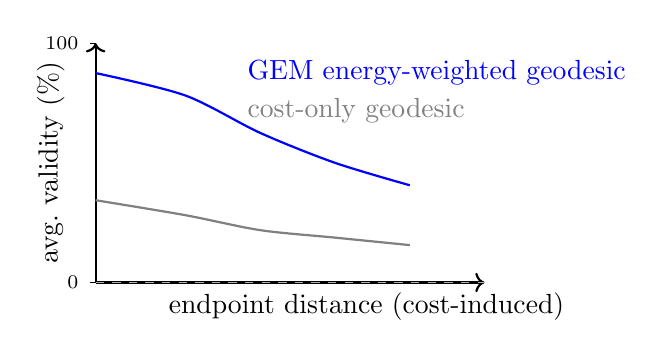
\begin{tikzpicture}[scale=0.95]
  \draw[->, thick] (0,0) -- (5.2,0) node[below, xshift=-1.5cm] {endpoint distance (cost-induced)};
  \draw[->, thick] (0,0) -- (0,3.2);
  \node[rotate=90] at (-0.6,1.6) {avg.\ validity (\%)};

  \draw (0,0) -- (-0.08,0);
  \node[left, font=\scriptsize] at (-0.1,0) {0};
  \draw (0,3.2) -- (-0.08,3.2);
  \node[left, font=\scriptsize] at (-0.1,3.2) {100};

  \draw[gray!60, dashed] (0,0) -- (5.2,0);

  \draw[thick, blue] plot[smooth] coordinates {(0.0,2.8) (1.2,2.5) (2.2,2.0) (3.2,1.6) (4.2,1.3)};
  \draw[thick, gray] plot[smooth] coordinates {(0.0,1.1) (1.2,0.9) (2.2,0.7) (3.2,0.6) (4.2,0.5)};

  \node[blue, anchor=west] at (1.9,2.8) {GEM energy-weighted geodesic};
  \node[gray, anchor=west] at (1.9,2.3) {cost-only geodesic};
\end{tikzpicture}
\caption{\footnotesize \textbf{Validity Along Geodesics.} Expected average validity vs.\ endpoint distance (cost-induced) for GEM energy-weighted versus cost-only geodesics.}
\label{fig:geodesic-validity}
\end{figure}

%\section{Discussion: Remove parts into experiments and rest in conclusion TODO}
%\gls{gem} matches or exceed baseline models for molecular graph benchmarks in both the unconditional and conditional setting. It enables compositional, inference-time control by adding energy terms, as shown in the conditional
%experiments (Section~\ref{sec:experiments}). The learned energy also enables interpretable diagnostics,
%including geodesic analysis and likelihood-ratio calibration.

%\paragraph{Limitations} At very small inference budgets, diffusion-based baselines can reach strong performance with fewer steps;
%Figure~\ref{fig:moses-vun-steps} shows that in the few-step regime our current \gls{gem} sampler trails the
%diffusion baseline. More broadly, \glspl{ebm} for generation rely on gradient-based velocity parameterization,
%which typically requires both forward and backward passes per step and implies an inherent $\sim$2--3$\times$
%theoretical slowdown relative to purely forward samplers.


%\paragraph{Future directions} 
%A promising extension is 3D molecular generation: GEM can retain a strong graph prior while adding geometric energies such as distance/torsion constraints or pharmacophore terms at inference time. Additionally, GEM’s explicit energy landscape could be used for a broader diagnostics toolkit: relative likelihood rankings and
%energy-weighted geodesics can be used to quantify generalization or flag out-of-distribution regions. In particular, if the minimum-energy geodesic between two molecular (scaffold) families has a high-energy barrier, the model likely has low support (is effectively out-of-distribution) in the intermediates, so generations requiring that edit transition should be treated as low-trust.


%Old
%An immediate extension is 3D molecule generation, composing a strong graph prior with geometric
%constraints at inference time. Relative likelihoods can support scalable refinement and
%generalization diagnostics by testing energy rankings on held-out regions.

\section{Conclusion}
We introduced \emph{Graph Energy Matching} (GEM), a framework motivated by the map-optimization perspective of the \gls{jko} scheme, extending continuous energy matching principles to discrete graph spaces. GEM integrates deterministic, transport-aligned graph edits guiding sampling toward high-probability regions, with principled \gls{mcmc} mixing under a unified, scalar energy model, bridging graph generation and discrete energy-based modeling. This design provides two practical advantages: (i) scalable, high-quality unconditional molecular generation from both noise-initialized and data-driven (editing) initializations, and (ii) flexible inference-time conditional generation together with a learned relative-likelihood structure, enabling downstream tasks such as geodesic interpolation. Empirically, GEM is on pair or better against strong diffusion/\gls{ctmc} baselines on MOSES and QM9, and it performs effective property optimization under threshold constraints. Beyond generation quality, GEM exposes an explicit energy landscape that can be utilized for relative likelihood comparisons and geodesic analyses, providing a complementary diagnostic view of model support and controllability in learned molecular space. 

\paragraph{Limitations}: Broadly, \glspl{ebm} for generation rely on gradient-based velocity parameterization,
which typically requires both forward and backward passes per step and implies an inherent $\sim$2--3$\times$
theoretical slowdown relative to purely forward samplers. While gradient-based guidance and multi-step sampling introduce additional compute relative to purely forward generators, GEM offers a flexible and analyzable foundation for controllable graph generation.

\paragraph{Future Directions}:
A promising extension is 3D molecular generation: GEM can retain a strong graph prior while adding geometric energies such as distance or torsion constraints at inference time. Additionally, GEM’s explicit energy landscape offers a valuable diagnostics toolkit: by comparing energy profiles across datasets, one can directly quantify generalization to unseen distributions or flag out-of-distribution regions.

\FloatBarrier

%BIBLIOGRAPHY
\bibliographystyle{icml2026}
\bibliography{main}

%APPENDIX
\appendix
\section{Permutation-invariant minibatch matching}
\label{app:matching}

Exact computation of the \gls{fgw} cost $c_{\mathrm{FGW}}$ requires a combinatorial search over
permutations. We therefore use fast, permutation-invariant hard-assignment approximations
tailored to the source distribution and the downstream use (pairing vs.\ local edits).

\paragraph{Histogram matching for a uniform source.}
When the source $\pi_0$ is a uniform distribution over node and edge classes, we use a cheap signature
for each graph. Let $h_\mathcal{V}$ be the normalized node-type histogram, $h_\mathcal{E}$ the normalized edge-type
histogram (over $i<j$), and $h_{\mathcal{V}\mathcal{E}}$ the histogram over unordered node-type pairs with edge types. We
form a weighted signature $h(x)=[\alpha_1 h_\mathcal{V},\;\alpha_2 h_\mathcal{E},\;\alpha_3 h_{\mathcal{V}\mathcal{E}}]$ and solve a linear assignment
between graphs of equal size using $\|h(x)-h(y)\|_1$. This produces permutation-invariant couplings and
is sufficient when $\pi_0$ is far from $\pi_{\mathrm{data}}$, so we do not require fine-grained alignment.

\paragraph{Node matching for molecule-like sources.}
If the source distribution already produces valid molecules, we recommend a node-matching alignment
based on node labels (optionally with a light edge-structure tie-breaker), followed by computing the
aligned local cost. This reflects chemical atom mapping practice: once atoms are aligned, bond
correspondences are largely determined~\citep{bell2019dockrmsd}.

\section{Time weighting for the flow loss}
\label{app:flow-weighting}

The flow-matching term can be reweighted in time by introducing a scalar
$\alpha(t)$:
\begin{equation}
\mathcal{L}_{\text{flow},\alpha}(\theta)
=
\mathbb{E}_{(x_0,x_1)\sim\tilde{\gamma},\,t\sim\Unif([0,1])}\left[
\alpha(t)\,\|-\nabla_{\hat{x}} V_\theta(\hat{x}_t)-v\|_2^2
\right].
\end{equation}
A simple choice is a piecewise linear schedule
\begin{equation}
\alpha_{\tau^\ast}(t)=
\begin{cases}
1,&0\le t\le\tau^\ast,\\[6pt]
\dfrac{1-t}{1-\tau^\ast},&\tau^\ast<t\le1,
\end{cases}
\end{equation}
so that $\alpha_{\tau^\ast}(1)=0$. This downweights flow supervision for samples
approaching the data manifold and can reduce interference with $\mathcal{L}_{\text{ER}}$.
We do not apply this weighting in our experiments ($\alpha(t)\equiv 1$), because
full flow supervision was empirically more stable for $\mathcal{L}_{\text{ER}}$.

Time-decaying weights are common in continuous settings: Energy Matching and
Equilibrium Matching relax the flow term to avoid over-constraining the
equilibrium regime. In particular, Equilibrium Matching uses $\alpha(t)\to 0$
as $t\to 1$ because a vanishing energy gradient at equilibrium is one of the
score-matching conditions for energy-based training~\citep{wang2025equilibrium}.
Such schedules may be beneficial in other domains where late-time supervision
conflicts with equilibrium refinement.

\section{Geodesic analysis details}
\label{app:geodesic-details}

\paragraph{Pairing and alignments.}
We draw 1000 molecules from the dataset and group them by node count. For each group we sample
pairs uniformly and align them using node matching to define a coupling between endpoints.

\paragraph{Path optimization.}
We represent a continuous path in the embedding space and optimize the energy-weighted length
objective in \Cref{sec:experiments}, including the path-energy term. The linear baseline uses the
same endpoint pairing and interpolates between the coupled graphs.

\paragraph{Spline parameterization.}
We implement geodesic paths using a Bezier spline over learnable control-point logits for nodes and
edges. The spline lives in the probability simplex (node/edge categorical distributions), and
discrete graphs are sampled only for visualization and metric evaluation. The optimization minimizes
the relative length ratio $L_{\mathrm{spline}}/L_{\mathrm{linear}} - 1$, where the segment lengths are
weighted by $\exp(-\beta V_\theta(x_\tau))$ along the path.

\paragraph{Discrete evaluation.}
We discretize each continuous path at evenly spaced points in normalized arc length. At each point
we sample categorical graphs from the path distribution to compute validity and energy statistics.
We report the length ratio $L_{\mathrm{geo}}/L_{\mathrm{lin}}$ and the correlation between energy
and validity along the path.

\section{Contrastive loss objective derivation}\label{app:energy-refinement}
Given the model density (where $\beta_{\mathrm{mh}}$ is a constant):
\begin{equation}
p_\theta(x)=\frac{e^{-\beta_{\mathrm{mh}} V_\theta(x)}}{Z_\theta},
\qquad
Z_\theta=\sum_x e^{-\beta_{\mathrm{mh}} V_\theta(x)}.
\end{equation}
let us consider maximum likelihood estimation:
\begin{equation}
\theta^\star=\arg\max_\theta\;\mathbb{E}_{x\sim p_{\text{data}}}\big[\log p_\theta(x)\big]
\;\;\Longleftrightarrow\;\;
\theta^\star=\arg\min_\theta\;\mathcal{J}(\theta),
\end{equation}
with
\begin{equation}
\mathcal{J}(\theta):=-\mathbb{E}_{p_{\text{data}}}\big[\log p_\theta(x)\big]
=\mathbb{E}_{p_{\text{data}}}\big[\beta_{\mathrm{mh}} V_\theta(x)\big]+\log Z_\theta.
\end{equation}
Taking gradients gives
\begin{equation}
\nabla_\theta \mathcal{J}(\theta)
=\mathbb{E}_{p_{\text{data}}}\big[\beta_{\mathrm{mh}}\nabla_\theta V_\theta(x)\big]
+\nabla_\theta \log Z_\theta,
\end{equation}
where
\begin{equation}
\begin{aligned}
\nabla_\theta \log Z_\theta
&=\frac{1}{Z_\theta}\nabla_\theta Z_\theta
=\frac{1}{Z_\theta}\sum_x e^{-\beta_{\mathrm{mh}} V_\theta(x)}\big(-\beta_{\mathrm{mh}}\nabla_\theta V_\theta(x)\big)\\
&=-\mathbb{E}_{p_\theta}\big[\beta_{\mathrm{mh}}\nabla_\theta V_\theta(x)\big].
\end{aligned}
\end{equation}
Therefore, the gradient simplifies to
\begin{equation}
\boxed{
\nabla_\theta \mathcal{J}(\theta)
=\beta_{\mathrm{mh}}\left(\mathbb{E}_{p_{\text{data}}}\big[\nabla_\theta V_\theta(x)\big]
-\mathbb{E}_{p_\theta}\big[\nabla_\theta V_\theta(x)\big]\right)
}.
\end{equation}
This motivates the contrastive loss objective \(\mathcal{L}_{\mathrm{CL}}\) introduced in \eqref{eq:cl}, where we approximate the expectation over \(p_\theta\) using samples initialized either at uniform noise and data samples in 50\%/50\% proportions for general training, or exclusively at data samples (0\%/100\%) for the specialized training of data-initialized unconditional generation models. We then iteratively run a sequence of \((\text{greedy} + N_{\mathrm{CL}})\) proposals, explicitly detaching gradients flowing through the sampler transitions (i.e., Markov chain proposal and acceptance steps) to avoid backpropagation through the stochastic sampling process itself, ensuring stable estimation.

\section{Permutation-invariant energy parameterization}\label{app:perm-invariance}
FIME: Check notation and masking/padding
We implement the potential with a node/edge/global graph transformer backbone
(the GraphTransformer used in our codebase). Each layer is permutation equivariant:
for any relabeling $\sigma$, hidden node and edge features transform as
$(X,E)\mapsto (\sigma\!\cdot\!X,\sigma\!\cdot\!E)$. The global feature $h$ collects
extra graph-level features and is updated through permutation-invariant summaries,
so $h$ is invariant.

Here, $n$ denotes the maximum number of nodes observed in the training dataset; smaller graphs are padded and masked following standard conventions for graph diffusion models~\citep{vignac2022digress,qinmadeira2024defog}.

\begin{figure}[h]
\centering
\resizebox{\columnwidth}{!}{%
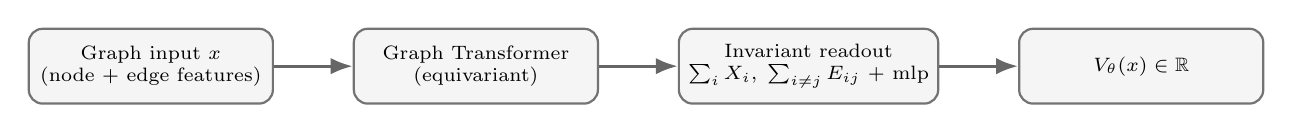
\begin{tikzpicture}[
  font=\scriptsize,
  node distance=1.0cm,
  module/.style={
    rectangle,
    rounded corners=5pt,
    minimum width=3.1cm,
    minimum height=0.95cm,
    align=center,
    draw=black!55,
    fill=black!4,
    thick
  },
  arrow/.style={-Latex, line width=1.1pt, draw=black!60}
]
  \node[module] (graph) {Graph input $x$\\(node + edge features)};
  \node[module, right=of graph] (gt) {Graph Transformer\\(equivariant)};
  \node[module, right=of gt] (pool) {Invariant readout\\$\sum_i X_i,\;\sum_{i\ne j} E_{ij}$ + \glsentryshort{mlp}};
  \node[module, right=of pool] (energy) {$V_\theta(x)\in\mathbb{R}$};

  \draw[arrow] (graph) -- (gt);
  \draw[arrow] (gt) -- (pool);
  \draw[arrow] (pool) -- (energy);
\end{tikzpicture}}
\caption{\textbf{Energy Backbone.} Permutation-equivariant backbone with invariant pooling to produce a scalar energy.}
\label{fig:energy-arch}
\end{figure}

The scalar energy is obtained by an invariant readout that first pools the
equivariant features and then applies an \gls{mlp}:
\begin{equation}
\begin{aligned}
\bar{X} &= \sum_{i\in\mathcal{V}} X^{(L)}_i,\qquad
\bar{E} = \sum_{i\ne j} E^{(L)}_{ij},\\
V_\theta(x,h) &= \mathrm{MLP}\big([\bar{X},\bar{E},h^{(L)}]\big).
\end{aligned}
\end{equation}
The sums are invariant to permutations, so the concatenated vector
$(\bar{X},\bar{E},h^{(L)})$ is invariant. Therefore any \gls{mlp} applied to it is
also invariant. This matches the sum-pooled energy head in the implementation
(with a masked off-diagonal sum).

\section{Conceptualizing baselines}
\label{app:baselines}

We summarize the baseline methods used in our experiments with an emphasis on the generation/sampling mechanism for each method. 

\paragraph{GraphEBM} ~\citep{liu2021graphebm} models molecular graphs using an energy-based model that assigns a scalar energy $E_\theta(x)$ to each graph $x$ via a graph neural network.
Unlike transport- or flow-based approaches, GraphEBM does not learn an explicit transformation from a source distribution to the data distribution. Instead, generation depends exclusively on Langevin dynamics sampling within a continuous embedding space.


\paragraph{DeFoG}~\citep{qinmadeira2024defog} adapts discrete flow matching to graphs by pairing an explicit noising path (via linear interpolation toward a simple base distribution) with a learned \gls{ctmc} denoiser: a network predicts the clean-graph posterior from an intermediate noisy graph, which in turn defines the time-dependent rate matrices used for generation.
Sampling starts from the base distribution and simulates the resulting \gls{ctmc} toward the data distribution, with the sampling step schedule largely selectable at inference time.

\paragraph{\gls{vfm}}~\citep{eijkelboom2024vfm} casts flow matching as variational inference over trajectory endpoints (the “posterior probability path”), yielding a KL-based objective that for categorical graph variables reduces to a per-component cross-entropy.
In contrast to DeFoG’s stochastic \gls{ctmc} jump dynamics, \gls{vfm} targets a deterministic continuous flow (vector field) on the probability simplex and generates by integrating this flow from the base distribution, then discretizing/sampling from the final categorical probabilities.


\paragraph{G-\gls{vfm}}~\citep{eijkelboom2025controlledvfm} extends \gls{vfm} with equivariant conditioning mechanisms to
support controllable generation.

\section{Sampling proposals}\label{app:sampling}

Figure~\ref{fig:appendix-mcmc-traj} provides a schematic of molecular graph evolution under \gls{mcmc}
steps for \gls{gem} on QM9 and MOSES.

\begin{figure*}[h]
\centering
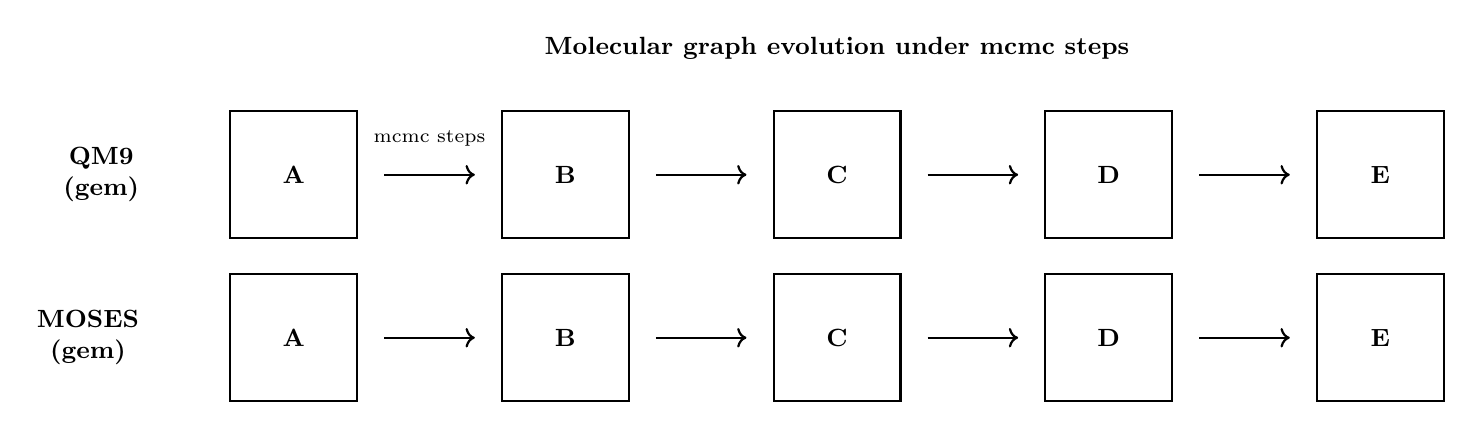
\begin{tikzpicture}[scale=1.15]
  % Layout constants
  \def\boxsize{1.4}
  \def\gap{3.0}
  \def\rowgap{1.8}
  \def\arrowlen{1.0}

  \pgfmathsetmacro{\titlex}{2*\gap + 0.5*\boxsize}
  \node[font=\small\bfseries] at (\titlex,2.1) {Molecular graph evolution under \gls{mcmc} steps};

  % Row labels
  \node[anchor=east, align=center, font=\small\bfseries] at (-0.9,0.5*\boxsize) {QM9\\(\gls{gem})};
  \node[anchor=east, align=center, font=\small\bfseries] at (-0.9,-\rowgap+0.5*\boxsize) {MOSES\\(\gls{gem})};

  % Row 1 (QM9)
  \foreach \i/\lab in {0/A,1/B,2/C,3/D,4/E} {
    \draw[thick] (\i*\gap,0) rectangle ++(\boxsize,\boxsize);
    \node[font=\small\bfseries] at (\i*\gap+0.5*\boxsize,0.5*\boxsize) {\lab};
  }
  \foreach \i in {0,1,2,3} {
    \draw[->, thick]
      ({\i*\gap + 0.5*(\gap+\boxsize) - 0.5*\arrowlen}, {0.5*\boxsize})
      -- ({\i*\gap + 0.5*(\gap+\boxsize) + 0.5*\arrowlen}, {0.5*\boxsize});
  }
  \node[font=\scriptsize] at ({0.5*(\gap+\boxsize)}, {0.5*\boxsize+0.4}) {\gls{mcmc} steps};

  % Row 2 (MOSES)
  \foreach \i/\lab in {0/A,1/B,2/C,3/D,4/E} {
    \draw[thick] (\i*\gap,-\rowgap) rectangle ++(\boxsize,\boxsize);
    \node[font=\small\bfseries] at (\i*\gap+0.5*\boxsize,-\rowgap+0.5*\boxsize) {\lab};
  }
  \foreach \i in {0,1,2,3} {
    \draw[->, thick]
      ({\i*\gap + 0.5*(\gap+\boxsize) - 0.5*\arrowlen}, {-\rowgap+0.5*\boxsize})
      -- ({\i*\gap + 0.5*(\gap+\boxsize) + 0.5*\arrowlen}, {-\rowgap+0.5*\boxsize});
  }
\end{tikzpicture}
\caption{\footnotesize \textbf{\gls{mcmc} Evolution.} Molecular graph evolution under \gls{mcmc} steps for \gls{gem} on QM9 and MOSES. \textcolor{red}{[WiP]}}
\label{fig:appendix-mcmc-traj}
\end{figure*}

\section{Unconditional generation on QM9}
\label{app:qm9-uncond}

QM9 unconditional metrics are reported in the main text (Table~\ref{tab:uncond-qm9}). V.U. is
saturated around 100\%, and lower FCD is often paid for with decreased novelty or larger networks
that can memorize the dataset.
\FloatBarrier

\section{Noise sensitivity of property regressors}
\label{app:regressor-noise}

Property regressors are trained on clean molecules, so evaluating them on noisy graphs is
ill-posed when bonds and valences are corrupted. We measure the degradation by computing test
MAE as a function of noise level $t$ along the diffusion path. We use 10k test molecules and
report three representative properties (SAS, logS, QED). As expected, errors are large for
noisy inputs and only become reasonable at $t=1$ (fully denoised, clean samples).
Figure~\ref{fig:regressor-noise} summarizes the trend.

\begin{figure}[H]
\centering
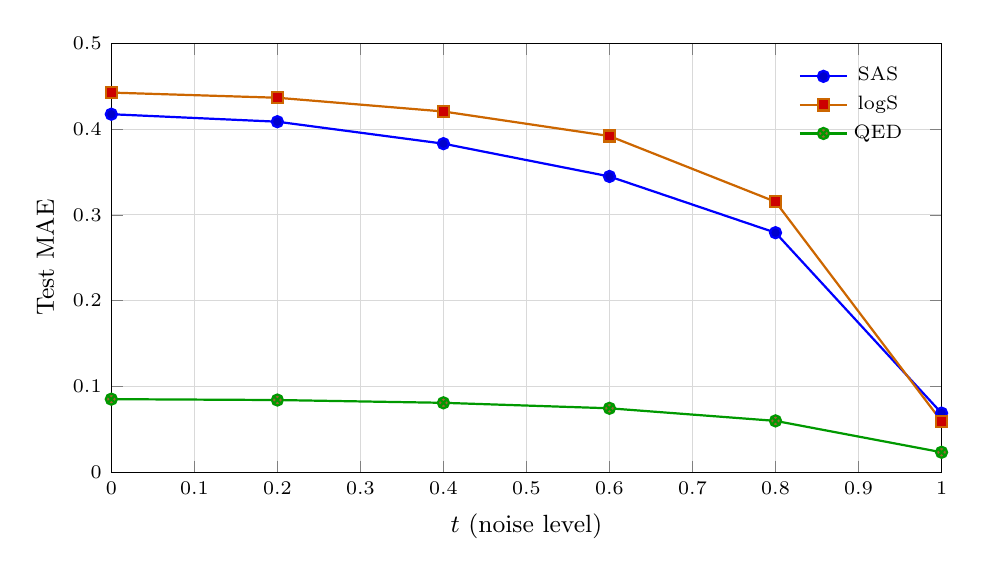
\begin{tikzpicture}
\begin{axis}[
  width=\columnwidth,
  height=0.58\columnwidth,
  xlabel={$t$ (noise level)},
  ylabel={Test MAE},
  xmin=0, xmax=1,
  ymin=0, ymax=0.5,
  grid=both,
  grid style={line width=0.3pt, draw=gray!30},
  tick label style={font=\scriptsize},
  label style={font=\small},
  legend style={font=\scriptsize, draw=none, fill=none},
  legend pos=north east,
]
\addplot+[thick, blue] coordinates {
  (0.0, 0.4171967224)
  (0.2, 0.4084696747)
  (0.4, 0.3828861816)
  (0.6, 0.3446883911)
  (0.8, 0.2791697571)
  (1.0, 0.0690200127)
};
\addlegendentry{SAS}

\addplot+[thick, orange!80!black] coordinates {
  (0.0, 0.4423901184)
  (0.2, 0.4363820099)
  (0.4, 0.4203746033)
  (0.6, 0.3917442139)
  (0.8, 0.3152096558)
  (1.0, 0.0594828186)
};
\addlegendentry{logS}

\addplot+[thick, green!60!black] coordinates {
  (0.0, 0.0852654148)
  (0.2, 0.0842592201)
  (0.4, 0.0810060917)
  (0.6, 0.0746299919)
  (0.8, 0.0599623322)
  (1.0, 0.0234130266)
};
\addlegendentry{QED}
\end{axis}
\end{tikzpicture}
\caption{\footnotesize Test MAE of time/noise-conditioned property regressors versus noise level $t$
(0 = fully noised, 1 = clean/denoised). Each point averages 10k test molecules. Errors are large for
noisy inputs and only reasonable at $t=1$.}
\label{fig:regressor-noise}
\end{figure}

\section{Hyperparameters}
\label{app:hyperparams}
We report the hyperparameters used for all runs here. \textcolor{red}{[WiP]}
We also report the diffusion-editing noise level $\tau$ selected for each baseline here. \textcolor{red}{[WiP]}

\section{Experimental setup}
\label{app:exp-setup}
We summarize datasets, preprocessing, training, and sampling settings here. \textcolor{red}{[WiP]}
\noindent\textit{Property optimization regressors.} Baselines use their standard marginal-noise
conditioning, while \gls{gem} uses uniform-noise conditioning (our training noise), with other settings
matched.

\end{document}
